\begin{figure}[H] \centering % Created by tikzDevice version 0.12.4 on 2023-07-24 17:06:23
% !TEX encoding = UTF-8 Unicode
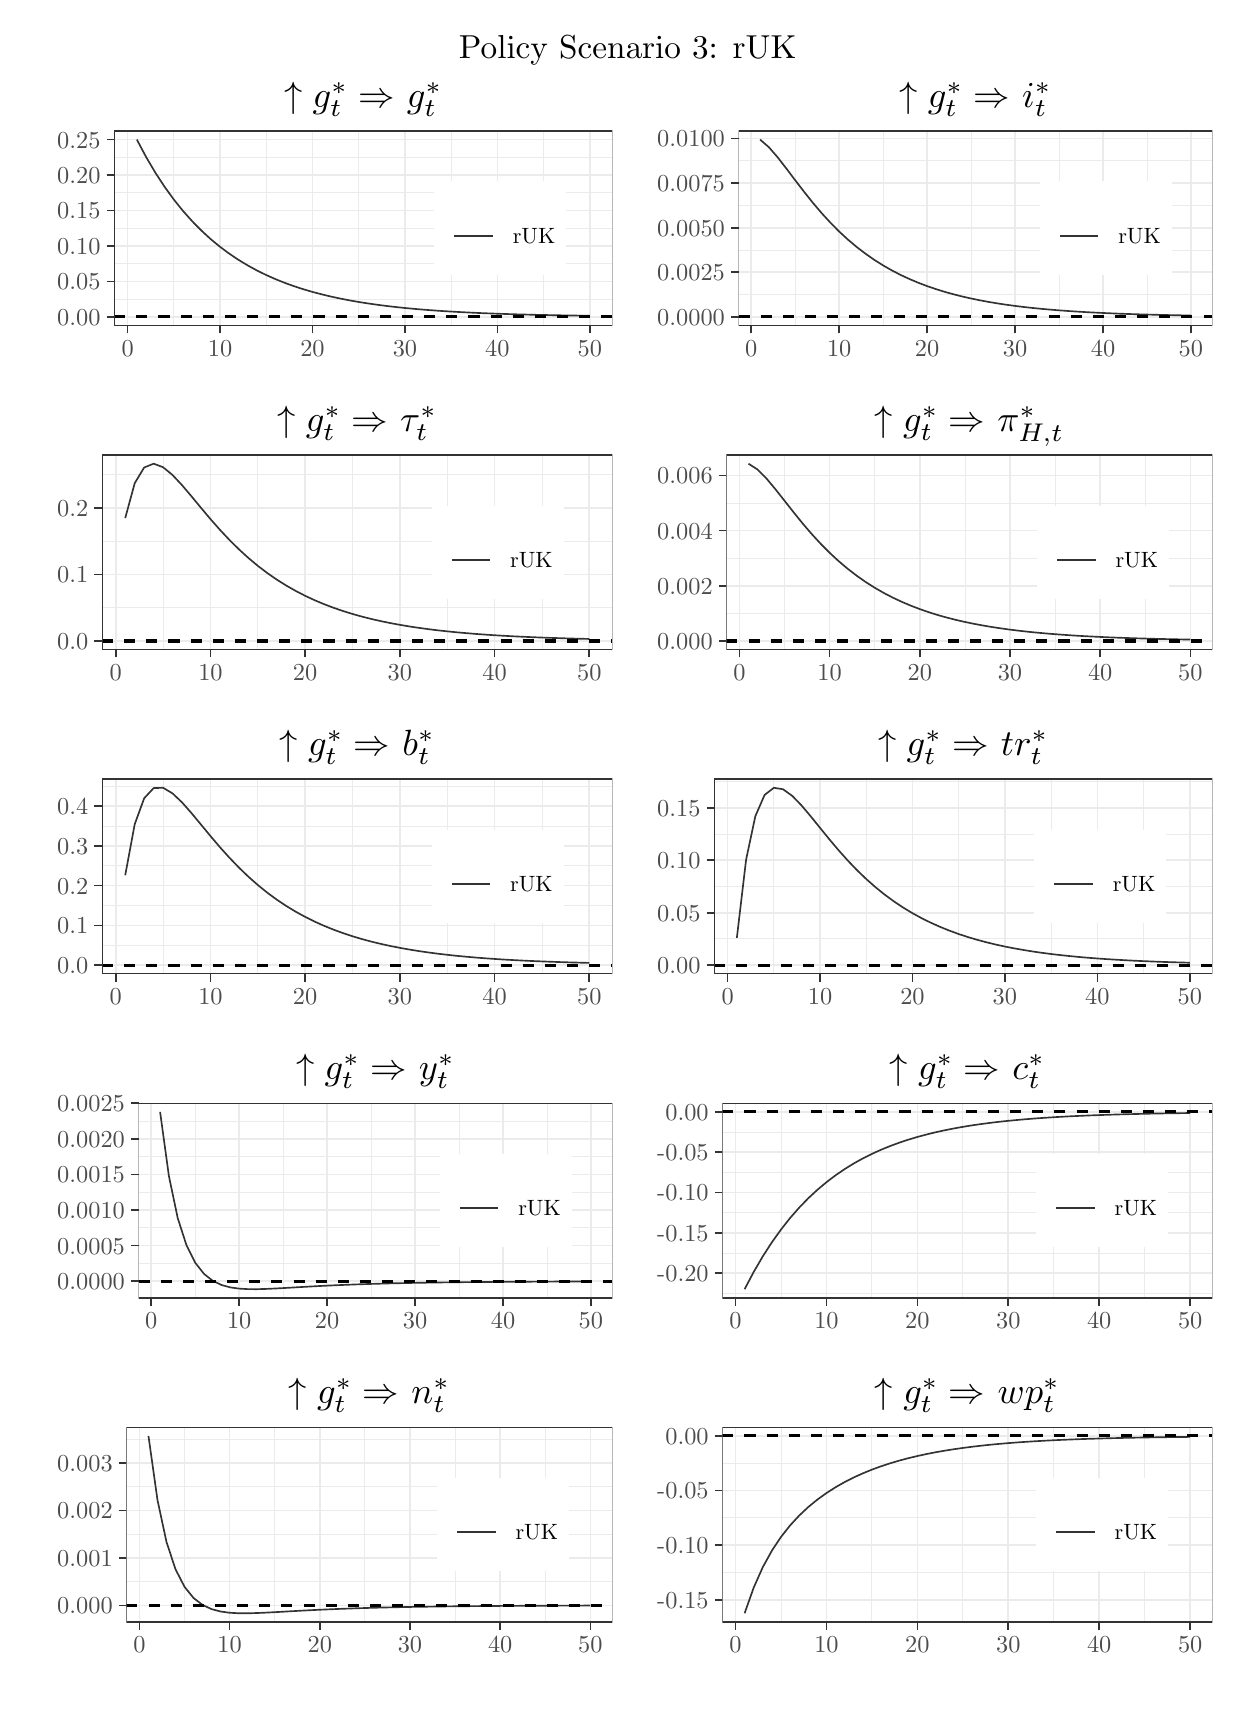
\begin{tikzpicture}[x=1pt,y=1pt]
\definecolor{fillColor}{RGB}{255,255,255}
\path[use as bounding box,fill=fillColor,fill opacity=0.00] (0,0) rectangle (433.62,599.84);
\begin{scope}
\path[clip] (  0.00,468.44) rectangle (216.81,585.55);
\definecolor{drawColor}{RGB}{255,255,255}
\definecolor{fillColor}{RGB}{255,255,255}

\path[draw=drawColor,line width= 0.6pt,line join=round,line cap=round,fill=fillColor] (  0.00,468.44) rectangle (216.81,585.55);
\end{scope}
\begin{scope}
\path[clip] ( 31.27,492.12) rectangle (211.31,562.59);
\definecolor{fillColor}{RGB}{255,255,255}

\path[fill=fillColor] ( 31.27,492.12) rectangle (211.31,562.59);
\definecolor{drawColor}{gray}{0.92}

\path[draw=drawColor,line width= 0.3pt,line join=round] ( 31.27,501.73) --
	(211.31,501.73);

\path[draw=drawColor,line width= 0.3pt,line join=round] ( 31.27,514.54) --
	(211.31,514.54);

\path[draw=drawColor,line width= 0.3pt,line join=round] ( 31.27,527.36) --
	(211.31,527.36);

\path[draw=drawColor,line width= 0.3pt,line join=round] ( 31.27,540.17) --
	(211.31,540.17);

\path[draw=drawColor,line width= 0.3pt,line join=round] ( 31.27,552.98) --
	(211.31,552.98);

\path[draw=drawColor,line width= 0.3pt,line join=round] ( 52.81,492.12) --
	( 52.81,562.59);

\path[draw=drawColor,line width= 0.3pt,line join=round] ( 86.22,492.12) --
	( 86.22,562.59);

\path[draw=drawColor,line width= 0.3pt,line join=round] (119.62,492.12) --
	(119.62,562.59);

\path[draw=drawColor,line width= 0.3pt,line join=round] (153.02,492.12) --
	(153.02,562.59);

\path[draw=drawColor,line width= 0.3pt,line join=round] (186.43,492.12) --
	(186.43,562.59);

\path[draw=drawColor,line width= 0.6pt,line join=round] ( 31.27,495.32) --
	(211.31,495.32);

\path[draw=drawColor,line width= 0.6pt,line join=round] ( 31.27,508.14) --
	(211.31,508.14);

\path[draw=drawColor,line width= 0.6pt,line join=round] ( 31.27,520.95) --
	(211.31,520.95);

\path[draw=drawColor,line width= 0.6pt,line join=round] ( 31.27,533.76) --
	(211.31,533.76);

\path[draw=drawColor,line width= 0.6pt,line join=round] ( 31.27,546.58) --
	(211.31,546.58);

\path[draw=drawColor,line width= 0.6pt,line join=round] ( 31.27,559.39) --
	(211.31,559.39);

\path[draw=drawColor,line width= 0.6pt,line join=round] ( 36.11,492.12) --
	( 36.11,562.59);

\path[draw=drawColor,line width= 0.6pt,line join=round] ( 69.52,492.12) --
	( 69.52,562.59);

\path[draw=drawColor,line width= 0.6pt,line join=round] (102.92,492.12) --
	(102.92,562.59);

\path[draw=drawColor,line width= 0.6pt,line join=round] (136.32,492.12) --
	(136.32,562.59);

\path[draw=drawColor,line width= 0.6pt,line join=round] (169.72,492.12) --
	(169.72,562.59);

\path[draw=drawColor,line width= 0.6pt,line join=round] (203.13,492.12) --
	(203.13,562.59);
\definecolor{drawColor}{gray}{0.20}

\path[draw=drawColor,line width= 0.6pt,line join=round] ( 39.45,559.39) --
	( 42.79,553.11) --
	( 46.13,547.45) --
	( 49.47,542.34) --
	( 52.81,537.73) --
	( 56.15,533.58) --
	( 59.50,529.83) --
	( 62.84,526.45) --
	( 66.18,523.39) --
	( 69.52,520.64) --
	( 72.86,518.16) --
	( 76.20,515.92) --
	( 79.54,513.91) --
	( 82.88,512.08) --
	( 86.22,510.44) --
	( 89.56,508.96) --
	( 92.90,507.62) --
	( 96.24,506.42) --
	( 99.58,505.33) --
	(102.92,504.35) --
	(106.26,503.47) --
	(109.60,502.67) --
	(112.94,501.95) --
	(116.28,501.30) --
	(119.62,500.71) --
	(122.96,500.19) --
	(126.30,499.71) --
	(129.64,499.28) --
	(132.98,498.89) --
	(136.32,498.54) --
	(139.66,498.23) --
	(143.00,497.94) --
	(146.34,497.69) --
	(149.68,497.45) --
	(153.02,497.25) --
	(156.36,497.06) --
	(159.70,496.89) --
	(163.04,496.73) --
	(166.38,496.60) --
	(169.72,496.47) --
	(173.06,496.36) --
	(176.40,496.26) --
	(179.74,496.17) --
	(183.08,496.08) --
	(186.43,496.01) --
	(189.77,495.94) --
	(193.11,495.88) --
	(196.45,495.83) --
	(199.79,495.78) --
	(203.13,495.73);
\definecolor{drawColor}{RGB}{0,0,0}

\path[draw=drawColor,line width= 1.1pt,dash pattern=on 4pt off 4pt ,line join=round] ( 31.27,495.32) -- (211.31,495.32);
\definecolor{drawColor}{gray}{0.20}

\path[draw=drawColor,line width= 0.6pt,line join=round,line cap=round] ( 31.27,492.12) rectangle (211.31,562.59);
\end{scope}
\begin{scope}
\path[clip] (  0.00,  0.00) rectangle (433.62,599.84);
\definecolor{drawColor}{gray}{0.30}

\node[text=drawColor,anchor=base east,inner sep=0pt, outer sep=0pt, scale=  0.88] at ( 26.32,492.29) {0.00};

\node[text=drawColor,anchor=base east,inner sep=0pt, outer sep=0pt, scale=  0.88] at ( 26.32,505.11) {0.05};

\node[text=drawColor,anchor=base east,inner sep=0pt, outer sep=0pt, scale=  0.88] at ( 26.32,517.92) {0.10};

\node[text=drawColor,anchor=base east,inner sep=0pt, outer sep=0pt, scale=  0.88] at ( 26.32,530.73) {0.15};

\node[text=drawColor,anchor=base east,inner sep=0pt, outer sep=0pt, scale=  0.88] at ( 26.32,543.55) {0.20};

\node[text=drawColor,anchor=base east,inner sep=0pt, outer sep=0pt, scale=  0.88] at ( 26.32,556.36) {0.25};
\end{scope}
\begin{scope}
\path[clip] (  0.00,  0.00) rectangle (433.62,599.84);
\definecolor{drawColor}{gray}{0.20}

\path[draw=drawColor,line width= 0.6pt,line join=round] ( 28.52,495.32) --
	( 31.27,495.32);

\path[draw=drawColor,line width= 0.6pt,line join=round] ( 28.52,508.14) --
	( 31.27,508.14);

\path[draw=drawColor,line width= 0.6pt,line join=round] ( 28.52,520.95) --
	( 31.27,520.95);

\path[draw=drawColor,line width= 0.6pt,line join=round] ( 28.52,533.76) --
	( 31.27,533.76);

\path[draw=drawColor,line width= 0.6pt,line join=round] ( 28.52,546.58) --
	( 31.27,546.58);

\path[draw=drawColor,line width= 0.6pt,line join=round] ( 28.52,559.39) --
	( 31.27,559.39);
\end{scope}
\begin{scope}
\path[clip] (  0.00,  0.00) rectangle (433.62,599.84);
\definecolor{drawColor}{gray}{0.20}

\path[draw=drawColor,line width= 0.6pt,line join=round] ( 36.11,489.37) --
	( 36.11,492.12);

\path[draw=drawColor,line width= 0.6pt,line join=round] ( 69.52,489.37) --
	( 69.52,492.12);

\path[draw=drawColor,line width= 0.6pt,line join=round] (102.92,489.37) --
	(102.92,492.12);

\path[draw=drawColor,line width= 0.6pt,line join=round] (136.32,489.37) --
	(136.32,492.12);

\path[draw=drawColor,line width= 0.6pt,line join=round] (169.72,489.37) --
	(169.72,492.12);

\path[draw=drawColor,line width= 0.6pt,line join=round] (203.13,489.37) --
	(203.13,492.12);
\end{scope}
\begin{scope}
\path[clip] (  0.00,  0.00) rectangle (433.62,599.84);
\definecolor{drawColor}{gray}{0.30}

\node[text=drawColor,anchor=base,inner sep=0pt, outer sep=0pt, scale=  0.88] at ( 36.11,481.11) {0};

\node[text=drawColor,anchor=base,inner sep=0pt, outer sep=0pt, scale=  0.88] at ( 69.52,481.11) {10};

\node[text=drawColor,anchor=base,inner sep=0pt, outer sep=0pt, scale=  0.88] at (102.92,481.11) {20};

\node[text=drawColor,anchor=base,inner sep=0pt, outer sep=0pt, scale=  0.88] at (136.32,481.11) {30};

\node[text=drawColor,anchor=base,inner sep=0pt, outer sep=0pt, scale=  0.88] at (169.72,481.11) {40};

\node[text=drawColor,anchor=base,inner sep=0pt, outer sep=0pt, scale=  0.88] at (203.13,481.11) {50};
\end{scope}
\begin{scope}
\path[clip] (  0.00,  0.00) rectangle (433.62,599.84);
\definecolor{fillColor}{RGB}{255,255,255}

\path[fill=fillColor] (146.96,510.43) rectangle (194.64,544.28);
\end{scope}
\begin{scope}
\path[clip] (  0.00,  0.00) rectangle (433.62,599.84);
\definecolor{fillColor}{RGB}{255,255,255}

\path[fill=fillColor] (152.46,515.93) rectangle (169.81,533.28);
\end{scope}
\begin{scope}
\path[clip] (  0.00,  0.00) rectangle (433.62,599.84);
\definecolor{drawColor}{gray}{0.20}

\path[draw=drawColor,line width= 0.6pt,line join=round] (154.20,524.61) -- (168.08,524.61);
\end{scope}
\begin{scope}
\path[clip] (  0.00,  0.00) rectangle (433.62,599.84);
\definecolor{drawColor}{RGB}{0,0,0}

\node[text=drawColor,anchor=base west,inner sep=0pt, outer sep=0pt, scale=  0.80] at (175.31,521.85) {rUK};
\end{scope}
\begin{scope}
\path[clip] (  0.00,  0.00) rectangle (433.62,599.84);
\definecolor{drawColor}{RGB}{0,0,0}

\node[text=drawColor,anchor=base,inner sep=0pt, outer sep=0pt, scale=  1.32] at (121.29,570.96) {$\uparrow  g^*_t \Rightarrow $ ${g^*_t}$};
\end{scope}
\begin{scope}
\path[clip] (216.81,468.44) rectangle (433.62,585.55);
\definecolor{drawColor}{RGB}{255,255,255}
\definecolor{fillColor}{RGB}{255,255,255}

\path[draw=drawColor,line width= 0.6pt,line join=round,line cap=round,fill=fillColor] (216.81,468.44) rectangle (433.62,585.55);
\end{scope}
\begin{scope}
\path[clip] (256.88,492.12) rectangle (428.12,562.59);
\definecolor{fillColor}{RGB}{255,255,255}

\path[fill=fillColor] (256.88,492.12) rectangle (428.12,562.59);
\definecolor{drawColor}{gray}{0.92}

\path[draw=drawColor,line width= 0.3pt,line join=round] (256.88,503.38) --
	(428.12,503.38);

\path[draw=drawColor,line width= 0.3pt,line join=round] (256.88,519.50) --
	(428.12,519.50);

\path[draw=drawColor,line width= 0.3pt,line join=round] (256.88,535.62) --
	(428.12,535.62);

\path[draw=drawColor,line width= 0.3pt,line join=round] (256.88,551.74) --
	(428.12,551.74);

\path[draw=drawColor,line width= 0.3pt,line join=round] (277.37,492.12) --
	(277.37,562.59);

\path[draw=drawColor,line width= 0.3pt,line join=round] (309.14,492.12) --
	(309.14,562.59);

\path[draw=drawColor,line width= 0.3pt,line join=round] (340.91,492.12) --
	(340.91,562.59);

\path[draw=drawColor,line width= 0.3pt,line join=round] (372.68,492.12) --
	(372.68,562.59);

\path[draw=drawColor,line width= 0.3pt,line join=round] (404.45,492.12) --
	(404.45,562.59);

\path[draw=drawColor,line width= 0.6pt,line join=round] (256.88,495.32) --
	(428.12,495.32);

\path[draw=drawColor,line width= 0.6pt,line join=round] (256.88,511.44) --
	(428.12,511.44);

\path[draw=drawColor,line width= 0.6pt,line join=round] (256.88,527.56) --
	(428.12,527.56);

\path[draw=drawColor,line width= 0.6pt,line join=round] (256.88,543.68) --
	(428.12,543.68);

\path[draw=drawColor,line width= 0.6pt,line join=round] (256.88,559.80) --
	(428.12,559.80);

\path[draw=drawColor,line width= 0.6pt,line join=round] (261.48,492.12) --
	(261.48,562.59);

\path[draw=drawColor,line width= 0.6pt,line join=round] (293.25,492.12) --
	(293.25,562.59);

\path[draw=drawColor,line width= 0.6pt,line join=round] (325.03,492.12) --
	(325.03,562.59);

\path[draw=drawColor,line width= 0.6pt,line join=round] (356.80,492.12) --
	(356.80,562.59);

\path[draw=drawColor,line width= 0.6pt,line join=round] (388.57,492.12) --
	(388.57,562.59);

\path[draw=drawColor,line width= 0.6pt,line join=round] (420.34,492.12) --
	(420.34,562.59);
\definecolor{drawColor}{gray}{0.20}

\path[draw=drawColor,line width= 0.6pt,line join=round] (264.66,559.39) --
	(267.84,556.63) --
	(271.02,552.97) --
	(274.19,548.88) --
	(277.37,544.67) --
	(280.55,540.53) --
	(283.72,536.56) --
	(286.90,532.82) --
	(290.08,529.35) --
	(293.25,526.15) --
	(296.43,523.22) --
	(299.61,520.55) --
	(302.79,518.12) --
	(305.96,515.91) --
	(309.14,513.91) --
	(312.32,512.10) --
	(315.49,510.46) --
	(318.67,508.99) --
	(321.85,507.65) --
	(325.03,506.44) --
	(328.20,505.36) --
	(331.38,504.37) --
	(334.56,503.49) --
	(337.73,502.69) --
	(340.91,501.97) --
	(344.09,501.32) --
	(347.26,500.73) --
	(350.44,500.20) --
	(353.62,499.72) --
	(356.80,499.29) --
	(359.97,498.90) --
	(363.15,498.55) --
	(366.33,498.23) --
	(369.50,497.95) --
	(372.68,497.69) --
	(375.86,497.46) --
	(379.03,497.25) --
	(382.21,497.06) --
	(385.39,496.89) --
	(388.57,496.74) --
	(391.74,496.60) --
	(394.92,496.47) --
	(398.10,496.36) --
	(401.27,496.26) --
	(404.45,496.17) --
	(407.63,496.09) --
	(410.81,496.01) --
	(413.98,495.94) --
	(417.16,495.88) --
	(420.34,495.83);
\definecolor{drawColor}{RGB}{0,0,0}

\path[draw=drawColor,line width= 1.1pt,dash pattern=on 4pt off 4pt ,line join=round] (256.88,495.32) -- (428.12,495.32);
\definecolor{drawColor}{gray}{0.20}

\path[draw=drawColor,line width= 0.6pt,line join=round,line cap=round] (256.88,492.12) rectangle (428.12,562.59);
\end{scope}
\begin{scope}
\path[clip] (  0.00,  0.00) rectangle (433.62,599.84);
\definecolor{drawColor}{gray}{0.30}

\node[text=drawColor,anchor=base east,inner sep=0pt, outer sep=0pt, scale=  0.88] at (251.93,492.29) {0.0000};

\node[text=drawColor,anchor=base east,inner sep=0pt, outer sep=0pt, scale=  0.88] at (251.93,508.41) {0.0025};

\node[text=drawColor,anchor=base east,inner sep=0pt, outer sep=0pt, scale=  0.88] at (251.93,524.53) {0.0050};

\node[text=drawColor,anchor=base east,inner sep=0pt, outer sep=0pt, scale=  0.88] at (251.93,540.65) {0.0075};

\node[text=drawColor,anchor=base east,inner sep=0pt, outer sep=0pt, scale=  0.88] at (251.93,556.77) {0.0100};
\end{scope}
\begin{scope}
\path[clip] (  0.00,  0.00) rectangle (433.62,599.84);
\definecolor{drawColor}{gray}{0.20}

\path[draw=drawColor,line width= 0.6pt,line join=round] (254.13,495.32) --
	(256.88,495.32);

\path[draw=drawColor,line width= 0.6pt,line join=round] (254.13,511.44) --
	(256.88,511.44);

\path[draw=drawColor,line width= 0.6pt,line join=round] (254.13,527.56) --
	(256.88,527.56);

\path[draw=drawColor,line width= 0.6pt,line join=round] (254.13,543.68) --
	(256.88,543.68);

\path[draw=drawColor,line width= 0.6pt,line join=round] (254.13,559.80) --
	(256.88,559.80);
\end{scope}
\begin{scope}
\path[clip] (  0.00,  0.00) rectangle (433.62,599.84);
\definecolor{drawColor}{gray}{0.20}

\path[draw=drawColor,line width= 0.6pt,line join=round] (261.48,489.37) --
	(261.48,492.12);

\path[draw=drawColor,line width= 0.6pt,line join=round] (293.25,489.37) --
	(293.25,492.12);

\path[draw=drawColor,line width= 0.6pt,line join=round] (325.03,489.37) --
	(325.03,492.12);

\path[draw=drawColor,line width= 0.6pt,line join=round] (356.80,489.37) --
	(356.80,492.12);

\path[draw=drawColor,line width= 0.6pt,line join=round] (388.57,489.37) --
	(388.57,492.12);

\path[draw=drawColor,line width= 0.6pt,line join=round] (420.34,489.37) --
	(420.34,492.12);
\end{scope}
\begin{scope}
\path[clip] (  0.00,  0.00) rectangle (433.62,599.84);
\definecolor{drawColor}{gray}{0.30}

\node[text=drawColor,anchor=base,inner sep=0pt, outer sep=0pt, scale=  0.88] at (261.48,481.11) {0};

\node[text=drawColor,anchor=base,inner sep=0pt, outer sep=0pt, scale=  0.88] at (293.25,481.11) {10};

\node[text=drawColor,anchor=base,inner sep=0pt, outer sep=0pt, scale=  0.88] at (325.03,481.11) {20};

\node[text=drawColor,anchor=base,inner sep=0pt, outer sep=0pt, scale=  0.88] at (356.80,481.11) {30};

\node[text=drawColor,anchor=base,inner sep=0pt, outer sep=0pt, scale=  0.88] at (388.57,481.11) {40};

\node[text=drawColor,anchor=base,inner sep=0pt, outer sep=0pt, scale=  0.88] at (420.34,481.11) {50};
\end{scope}
\begin{scope}
\path[clip] (  0.00,  0.00) rectangle (433.62,599.84);
\definecolor{fillColor}{RGB}{255,255,255}

\path[fill=fillColor] (365.75,510.43) rectangle (413.43,544.28);
\end{scope}
\begin{scope}
\path[clip] (  0.00,  0.00) rectangle (433.62,599.84);
\definecolor{fillColor}{RGB}{255,255,255}

\path[fill=fillColor] (371.25,515.93) rectangle (388.60,533.28);
\end{scope}
\begin{scope}
\path[clip] (  0.00,  0.00) rectangle (433.62,599.84);
\definecolor{drawColor}{gray}{0.20}

\path[draw=drawColor,line width= 0.6pt,line join=round] (372.99,524.61) -- (386.86,524.61);
\end{scope}
\begin{scope}
\path[clip] (  0.00,  0.00) rectangle (433.62,599.84);
\definecolor{drawColor}{RGB}{0,0,0}

\node[text=drawColor,anchor=base west,inner sep=0pt, outer sep=0pt, scale=  0.80] at (394.10,521.85) {rUK};
\end{scope}
\begin{scope}
\path[clip] (  0.00,  0.00) rectangle (433.62,599.84);
\definecolor{drawColor}{RGB}{0,0,0}

\node[text=drawColor,anchor=base,inner sep=0pt, outer sep=0pt, scale=  1.32] at (342.50,570.96) {$\uparrow  g^*_t \Rightarrow $ ${i^*_t}$};
\end{scope}
\begin{scope}
\path[clip] (  0.00,351.33) rectangle (216.81,468.44);
\definecolor{drawColor}{RGB}{255,255,255}
\definecolor{fillColor}{RGB}{255,255,255}

\path[draw=drawColor,line width= 0.6pt,line join=round,line cap=round,fill=fillColor] (  0.00,351.33) rectangle (216.81,468.44);
\end{scope}
\begin{scope}
\path[clip] ( 26.87,375.01) rectangle (211.31,445.48);
\definecolor{fillColor}{RGB}{255,255,255}

\path[fill=fillColor] ( 26.87,375.01) rectangle (211.31,445.48);
\definecolor{drawColor}{gray}{0.92}

\path[draw=drawColor,line width= 0.3pt,line join=round] ( 26.87,390.23) --
	(211.31,390.23);

\path[draw=drawColor,line width= 0.3pt,line join=round] ( 26.87,414.26) --
	(211.31,414.26);

\path[draw=drawColor,line width= 0.3pt,line join=round] ( 26.87,438.28) --
	(211.31,438.28);

\path[draw=drawColor,line width= 0.3pt,line join=round] ( 48.94,375.01) --
	( 48.94,445.48);

\path[draw=drawColor,line width= 0.3pt,line join=round] ( 83.16,375.01) --
	( 83.16,445.48);

\path[draw=drawColor,line width= 0.3pt,line join=round] (117.38,375.01) --
	(117.38,445.48);

\path[draw=drawColor,line width= 0.3pt,line join=round] (151.60,375.01) --
	(151.60,445.48);

\path[draw=drawColor,line width= 0.3pt,line join=round] (185.82,375.01) --
	(185.82,445.48);

\path[draw=drawColor,line width= 0.6pt,line join=round] ( 26.87,378.21) --
	(211.31,378.21);

\path[draw=drawColor,line width= 0.6pt,line join=round] ( 26.87,402.24) --
	(211.31,402.24);

\path[draw=drawColor,line width= 0.6pt,line join=round] ( 26.87,426.27) --
	(211.31,426.27);

\path[draw=drawColor,line width= 0.6pt,line join=round] ( 31.83,375.01) --
	( 31.83,445.48);

\path[draw=drawColor,line width= 0.6pt,line join=round] ( 66.05,375.01) --
	( 66.05,445.48);

\path[draw=drawColor,line width= 0.6pt,line join=round] (100.27,375.01) --
	(100.27,445.48);

\path[draw=drawColor,line width= 0.6pt,line join=round] (134.49,375.01) --
	(134.49,445.48);

\path[draw=drawColor,line width= 0.6pt,line join=round] (168.71,375.01) --
	(168.71,445.48);

\path[draw=drawColor,line width= 0.6pt,line join=round] (202.93,375.01) --
	(202.93,445.48);
\definecolor{drawColor}{gray}{0.20}

\path[draw=drawColor,line width= 0.6pt,line join=round] ( 35.25,422.62) --
	( 38.68,435.22) --
	( 42.10,440.91) --
	( 45.52,442.28) --
	( 48.94,441.00) --
	( 52.36,438.17) --
	( 55.79,434.51) --
	( 59.21,430.47) --
	( 62.63,426.33) --
	( 66.05,422.27) --
	( 69.47,418.39) --
	( 72.90,414.74) --
	( 76.32,411.35) --
	( 79.74,408.23) --
	( 83.16,405.37) --
	( 86.58,402.77) --
	( 90.00,400.40) --
	( 93.43,398.25) --
	( 96.85,396.31) --
	(100.27,394.54) --
	(103.69,392.95) --
	(107.11,391.51) --
	(110.54,390.21) --
	(113.96,389.04) --
	(117.38,387.98) --
	(120.80,387.02) --
	(124.22,386.16) --
	(127.65,385.38) --
	(131.07,384.68) --
	(134.49,384.05) --
	(137.91,383.47) --
	(141.33,382.96) --
	(144.75,382.49) --
	(148.18,382.07) --
	(151.60,381.70) --
	(155.02,381.35) --
	(158.44,381.05) --
	(161.86,380.77) --
	(165.29,380.52) --
	(168.71,380.29) --
	(172.13,380.09) --
	(175.55,379.90) --
	(178.97,379.74) --
	(182.40,379.59) --
	(185.82,379.45) --
	(189.24,379.33) --
	(192.66,379.22) --
	(196.08,379.12) --
	(199.50,379.03) --
	(202.93,378.95);
\definecolor{drawColor}{RGB}{0,0,0}

\path[draw=drawColor,line width= 1.1pt,dash pattern=on 4pt off 4pt ,line join=round] ( 26.87,378.21) -- (211.31,378.21);
\definecolor{drawColor}{gray}{0.20}

\path[draw=drawColor,line width= 0.6pt,line join=round,line cap=round] ( 26.87,375.01) rectangle (211.31,445.48);
\end{scope}
\begin{scope}
\path[clip] (  0.00,  0.00) rectangle (433.62,599.84);
\definecolor{drawColor}{gray}{0.30}

\node[text=drawColor,anchor=base east,inner sep=0pt, outer sep=0pt, scale=  0.88] at ( 21.92,375.18) {0.0};

\node[text=drawColor,anchor=base east,inner sep=0pt, outer sep=0pt, scale=  0.88] at ( 21.92,399.21) {0.1};

\node[text=drawColor,anchor=base east,inner sep=0pt, outer sep=0pt, scale=  0.88] at ( 21.92,423.24) {0.2};
\end{scope}
\begin{scope}
\path[clip] (  0.00,  0.00) rectangle (433.62,599.84);
\definecolor{drawColor}{gray}{0.20}

\path[draw=drawColor,line width= 0.6pt,line join=round] ( 24.12,378.21) --
	( 26.87,378.21);

\path[draw=drawColor,line width= 0.6pt,line join=round] ( 24.12,402.24) --
	( 26.87,402.24);

\path[draw=drawColor,line width= 0.6pt,line join=round] ( 24.12,426.27) --
	( 26.87,426.27);
\end{scope}
\begin{scope}
\path[clip] (  0.00,  0.00) rectangle (433.62,599.84);
\definecolor{drawColor}{gray}{0.20}

\path[draw=drawColor,line width= 0.6pt,line join=round] ( 31.83,372.26) --
	( 31.83,375.01);

\path[draw=drawColor,line width= 0.6pt,line join=round] ( 66.05,372.26) --
	( 66.05,375.01);

\path[draw=drawColor,line width= 0.6pt,line join=round] (100.27,372.26) --
	(100.27,375.01);

\path[draw=drawColor,line width= 0.6pt,line join=round] (134.49,372.26) --
	(134.49,375.01);

\path[draw=drawColor,line width= 0.6pt,line join=round] (168.71,372.26) --
	(168.71,375.01);

\path[draw=drawColor,line width= 0.6pt,line join=round] (202.93,372.26) --
	(202.93,375.01);
\end{scope}
\begin{scope}
\path[clip] (  0.00,  0.00) rectangle (433.62,599.84);
\definecolor{drawColor}{gray}{0.30}

\node[text=drawColor,anchor=base,inner sep=0pt, outer sep=0pt, scale=  0.88] at ( 31.83,364.00) {0};

\node[text=drawColor,anchor=base,inner sep=0pt, outer sep=0pt, scale=  0.88] at ( 66.05,364.00) {10};

\node[text=drawColor,anchor=base,inner sep=0pt, outer sep=0pt, scale=  0.88] at (100.27,364.00) {20};

\node[text=drawColor,anchor=base,inner sep=0pt, outer sep=0pt, scale=  0.88] at (134.49,364.00) {30};

\node[text=drawColor,anchor=base,inner sep=0pt, outer sep=0pt, scale=  0.88] at (168.71,364.00) {40};

\node[text=drawColor,anchor=base,inner sep=0pt, outer sep=0pt, scale=  0.88] at (202.93,364.00) {50};
\end{scope}
\begin{scope}
\path[clip] (  0.00,  0.00) rectangle (433.62,599.84);
\definecolor{fillColor}{RGB}{255,255,255}

\path[fill=fillColor] (145.97,393.32) rectangle (193.65,427.17);
\end{scope}
\begin{scope}
\path[clip] (  0.00,  0.00) rectangle (433.62,599.84);
\definecolor{fillColor}{RGB}{255,255,255}

\path[fill=fillColor] (151.47,398.82) rectangle (168.82,416.17);
\end{scope}
\begin{scope}
\path[clip] (  0.00,  0.00) rectangle (433.62,599.84);
\definecolor{drawColor}{gray}{0.20}

\path[draw=drawColor,line width= 0.6pt,line join=round] (153.21,407.50) -- (167.09,407.50);
\end{scope}
\begin{scope}
\path[clip] (  0.00,  0.00) rectangle (433.62,599.84);
\definecolor{drawColor}{RGB}{0,0,0}

\node[text=drawColor,anchor=base west,inner sep=0pt, outer sep=0pt, scale=  0.80] at (174.32,404.74) {rUK};
\end{scope}
\begin{scope}
\path[clip] (  0.00,  0.00) rectangle (433.62,599.84);
\definecolor{drawColor}{RGB}{0,0,0}

\node[text=drawColor,anchor=base,inner sep=0pt, outer sep=0pt, scale=  1.32] at (119.09,453.85) {$\uparrow  g^*_t \Rightarrow $ ${\tau^*_t}$};
\end{scope}
\begin{scope}
\path[clip] (216.81,351.33) rectangle (433.62,468.44);
\definecolor{drawColor}{RGB}{255,255,255}
\definecolor{fillColor}{RGB}{255,255,255}

\path[draw=drawColor,line width= 0.6pt,line join=round,line cap=round,fill=fillColor] (216.81,351.33) rectangle (433.62,468.44);
\end{scope}
\begin{scope}
\path[clip] (252.48,375.01) rectangle (428.12,445.48);
\definecolor{fillColor}{RGB}{255,255,255}

\path[fill=fillColor] (252.48,375.01) rectangle (428.12,445.48);
\definecolor{drawColor}{gray}{0.92}

\path[draw=drawColor,line width= 0.3pt,line join=round] (252.48,388.18) --
	(428.12,388.18);

\path[draw=drawColor,line width= 0.3pt,line join=round] (252.48,408.12) --
	(428.12,408.12);

\path[draw=drawColor,line width= 0.3pt,line join=round] (252.48,428.06) --
	(428.12,428.06);

\path[draw=drawColor,line width= 0.3pt,line join=round] (273.50,375.01) --
	(273.50,445.48);

\path[draw=drawColor,line width= 0.3pt,line join=round] (306.08,375.01) --
	(306.08,445.48);

\path[draw=drawColor,line width= 0.3pt,line join=round] (338.67,375.01) --
	(338.67,445.48);

\path[draw=drawColor,line width= 0.3pt,line join=round] (371.26,375.01) --
	(371.26,445.48);

\path[draw=drawColor,line width= 0.3pt,line join=round] (403.84,375.01) --
	(403.84,445.48);

\path[draw=drawColor,line width= 0.6pt,line join=round] (252.48,378.21) --
	(428.12,378.21);

\path[draw=drawColor,line width= 0.6pt,line join=round] (252.48,398.15) --
	(428.12,398.15);

\path[draw=drawColor,line width= 0.6pt,line join=round] (252.48,418.09) --
	(428.12,418.09);

\path[draw=drawColor,line width= 0.6pt,line join=round] (252.48,438.03) --
	(428.12,438.03);

\path[draw=drawColor,line width= 0.6pt,line join=round] (257.20,375.01) --
	(257.20,445.48);

\path[draw=drawColor,line width= 0.6pt,line join=round] (289.79,375.01) --
	(289.79,445.48);

\path[draw=drawColor,line width= 0.6pt,line join=round] (322.38,375.01) --
	(322.38,445.48);

\path[draw=drawColor,line width= 0.6pt,line join=round] (354.96,375.01) --
	(354.96,445.48);

\path[draw=drawColor,line width= 0.6pt,line join=round] (387.55,375.01) --
	(387.55,445.48);

\path[draw=drawColor,line width= 0.6pt,line join=round] (420.14,375.01) --
	(420.14,445.48);
\definecolor{drawColor}{gray}{0.20}

\path[draw=drawColor,line width= 0.6pt,line join=round] (260.46,442.28) --
	(263.72,440.19) --
	(266.98,436.90) --
	(270.24,433.00) --
	(273.50,428.87) --
	(276.76,424.73) --
	(280.01,420.71) --
	(283.27,416.91) --
	(286.53,413.36) --
	(289.79,410.08) --
	(293.05,407.06) --
	(296.31,404.31) --
	(299.57,401.80) --
	(302.82,399.52) --
	(306.08,397.45) --
	(309.34,395.58) --
	(312.60,393.89) --
	(315.86,392.36) --
	(319.12,390.98) --
	(322.38,389.73) --
	(325.64,388.60) --
	(328.89,387.58) --
	(332.15,386.67) --
	(335.41,385.84) --
	(338.67,385.09) --
	(341.93,384.42) --
	(345.19,383.81) --
	(348.45,383.26) --
	(351.70,382.77) --
	(354.96,382.32) --
	(358.22,381.92) --
	(361.48,381.55) --
	(364.74,381.23) --
	(368.00,380.93) --
	(371.26,380.67) --
	(374.52,380.43) --
	(377.77,380.21) --
	(381.03,380.01) --
	(384.29,379.84) --
	(387.55,379.68) --
	(390.81,379.53) --
	(394.07,379.40) --
	(397.33,379.29) --
	(400.58,379.18) --
	(403.84,379.09) --
	(407.10,379.00) --
	(410.36,378.92) --
	(413.62,378.85) --
	(416.88,378.79) --
	(420.14,378.73);
\definecolor{drawColor}{RGB}{0,0,0}

\path[draw=drawColor,line width= 1.1pt,dash pattern=on 4pt off 4pt ,line join=round] (252.48,378.21) -- (428.12,378.21);
\definecolor{drawColor}{gray}{0.20}

\path[draw=drawColor,line width= 0.6pt,line join=round,line cap=round] (252.48,375.01) rectangle (428.12,445.48);
\end{scope}
\begin{scope}
\path[clip] (  0.00,  0.00) rectangle (433.62,599.84);
\definecolor{drawColor}{gray}{0.30}

\node[text=drawColor,anchor=base east,inner sep=0pt, outer sep=0pt, scale=  0.88] at (247.53,375.18) {0.000};

\node[text=drawColor,anchor=base east,inner sep=0pt, outer sep=0pt, scale=  0.88] at (247.53,395.12) {0.002};

\node[text=drawColor,anchor=base east,inner sep=0pt, outer sep=0pt, scale=  0.88] at (247.53,415.06) {0.004};

\node[text=drawColor,anchor=base east,inner sep=0pt, outer sep=0pt, scale=  0.88] at (247.53,435.00) {0.006};
\end{scope}
\begin{scope}
\path[clip] (  0.00,  0.00) rectangle (433.62,599.84);
\definecolor{drawColor}{gray}{0.20}

\path[draw=drawColor,line width= 0.6pt,line join=round] (249.73,378.21) --
	(252.48,378.21);

\path[draw=drawColor,line width= 0.6pt,line join=round] (249.73,398.15) --
	(252.48,398.15);

\path[draw=drawColor,line width= 0.6pt,line join=round] (249.73,418.09) --
	(252.48,418.09);

\path[draw=drawColor,line width= 0.6pt,line join=round] (249.73,438.03) --
	(252.48,438.03);
\end{scope}
\begin{scope}
\path[clip] (  0.00,  0.00) rectangle (433.62,599.84);
\definecolor{drawColor}{gray}{0.20}

\path[draw=drawColor,line width= 0.6pt,line join=round] (257.20,372.26) --
	(257.20,375.01);

\path[draw=drawColor,line width= 0.6pt,line join=round] (289.79,372.26) --
	(289.79,375.01);

\path[draw=drawColor,line width= 0.6pt,line join=round] (322.38,372.26) --
	(322.38,375.01);

\path[draw=drawColor,line width= 0.6pt,line join=round] (354.96,372.26) --
	(354.96,375.01);

\path[draw=drawColor,line width= 0.6pt,line join=round] (387.55,372.26) --
	(387.55,375.01);

\path[draw=drawColor,line width= 0.6pt,line join=round] (420.14,372.26) --
	(420.14,375.01);
\end{scope}
\begin{scope}
\path[clip] (  0.00,  0.00) rectangle (433.62,599.84);
\definecolor{drawColor}{gray}{0.30}

\node[text=drawColor,anchor=base,inner sep=0pt, outer sep=0pt, scale=  0.88] at (257.20,364.00) {0};

\node[text=drawColor,anchor=base,inner sep=0pt, outer sep=0pt, scale=  0.88] at (289.79,364.00) {10};

\node[text=drawColor,anchor=base,inner sep=0pt, outer sep=0pt, scale=  0.88] at (322.38,364.00) {20};

\node[text=drawColor,anchor=base,inner sep=0pt, outer sep=0pt, scale=  0.88] at (354.96,364.00) {30};

\node[text=drawColor,anchor=base,inner sep=0pt, outer sep=0pt, scale=  0.88] at (387.55,364.00) {40};

\node[text=drawColor,anchor=base,inner sep=0pt, outer sep=0pt, scale=  0.88] at (420.14,364.00) {50};
\end{scope}
\begin{scope}
\path[clip] (  0.00,  0.00) rectangle (433.62,599.84);
\definecolor{fillColor}{RGB}{255,255,255}

\path[fill=fillColor] (364.76,393.32) rectangle (412.44,427.17);
\end{scope}
\begin{scope}
\path[clip] (  0.00,  0.00) rectangle (433.62,599.84);
\definecolor{fillColor}{RGB}{255,255,255}

\path[fill=fillColor] (370.26,398.82) rectangle (387.61,416.17);
\end{scope}
\begin{scope}
\path[clip] (  0.00,  0.00) rectangle (433.62,599.84);
\definecolor{drawColor}{gray}{0.20}

\path[draw=drawColor,line width= 0.6pt,line join=round] (372.00,407.50) -- (385.87,407.50);
\end{scope}
\begin{scope}
\path[clip] (  0.00,  0.00) rectangle (433.62,599.84);
\definecolor{drawColor}{RGB}{0,0,0}

\node[text=drawColor,anchor=base west,inner sep=0pt, outer sep=0pt, scale=  0.80] at (393.11,404.74) {rUK};
\end{scope}
\begin{scope}
\path[clip] (  0.00,  0.00) rectangle (433.62,599.84);
\definecolor{drawColor}{RGB}{0,0,0}

\node[text=drawColor,anchor=base,inner sep=0pt, outer sep=0pt, scale=  1.32] at (340.30,453.85) {$\uparrow  g^*_t \Rightarrow $ ${\pi^*_{H,t}}$};
\end{scope}
\begin{scope}
\path[clip] (  0.00,234.22) rectangle (216.81,351.33);
\definecolor{drawColor}{RGB}{255,255,255}
\definecolor{fillColor}{RGB}{255,255,255}

\path[draw=drawColor,line width= 0.6pt,line join=round,line cap=round,fill=fillColor] (  0.00,234.22) rectangle (216.81,351.33);
\end{scope}
\begin{scope}
\path[clip] ( 26.87,257.90) rectangle (211.31,328.37);
\definecolor{fillColor}{RGB}{255,255,255}

\path[fill=fillColor] ( 26.87,257.90) rectangle (211.31,328.37);
\definecolor{drawColor}{gray}{0.92}

\path[draw=drawColor,line width= 0.3pt,line join=round] ( 26.87,268.28) --
	(211.31,268.28);

\path[draw=drawColor,line width= 0.3pt,line join=round] ( 26.87,282.62) --
	(211.31,282.62);

\path[draw=drawColor,line width= 0.3pt,line join=round] ( 26.87,296.97) --
	(211.31,296.97);

\path[draw=drawColor,line width= 0.3pt,line join=round] ( 26.87,311.32) --
	(211.31,311.32);

\path[draw=drawColor,line width= 0.3pt,line join=round] ( 26.87,325.67) --
	(211.31,325.67);

\path[draw=drawColor,line width= 0.3pt,line join=round] ( 48.94,257.90) --
	( 48.94,328.37);

\path[draw=drawColor,line width= 0.3pt,line join=round] ( 83.16,257.90) --
	( 83.16,328.37);

\path[draw=drawColor,line width= 0.3pt,line join=round] (117.38,257.90) --
	(117.38,328.37);

\path[draw=drawColor,line width= 0.3pt,line join=round] (151.60,257.90) --
	(151.60,328.37);

\path[draw=drawColor,line width= 0.3pt,line join=round] (185.82,257.90) --
	(185.82,328.37);

\path[draw=drawColor,line width= 0.6pt,line join=round] ( 26.87,261.10) --
	(211.31,261.10);

\path[draw=drawColor,line width= 0.6pt,line join=round] ( 26.87,275.45) --
	(211.31,275.45);

\path[draw=drawColor,line width= 0.6pt,line join=round] ( 26.87,289.80) --
	(211.31,289.80);

\path[draw=drawColor,line width= 0.6pt,line join=round] ( 26.87,304.15) --
	(211.31,304.15);

\path[draw=drawColor,line width= 0.6pt,line join=round] ( 26.87,318.50) --
	(211.31,318.50);

\path[draw=drawColor,line width= 0.6pt,line join=round] ( 31.83,257.90) --
	( 31.83,328.37);

\path[draw=drawColor,line width= 0.6pt,line join=round] ( 66.05,257.90) --
	( 66.05,328.37);

\path[draw=drawColor,line width= 0.6pt,line join=round] (100.27,257.90) --
	(100.27,328.37);

\path[draw=drawColor,line width= 0.6pt,line join=round] (134.49,257.90) --
	(134.49,328.37);

\path[draw=drawColor,line width= 0.6pt,line join=round] (168.71,257.90) --
	(168.71,328.37);

\path[draw=drawColor,line width= 0.6pt,line join=round] (202.93,257.90) --
	(202.93,328.37);
\definecolor{drawColor}{gray}{0.20}

\path[draw=drawColor,line width= 0.6pt,line join=round] ( 35.25,293.57) --
	( 38.68,312.00) --
	( 42.10,321.39) --
	( 45.52,325.06) --
	( 48.94,325.17) --
	( 52.36,323.13) --
	( 55.79,319.88) --
	( 59.21,316.00) --
	( 62.63,311.87) --
	( 66.05,307.73) --
	( 69.47,303.71) --
	( 72.90,299.91) --
	( 76.32,296.35) --
	( 79.74,293.06) --
	( 83.16,290.04) --
	( 86.58,287.27) --
	( 90.00,284.76) --
	( 93.43,282.47) --
	( 96.85,280.40) --
	(100.27,278.52) --
	(103.69,276.82) --
	(107.11,275.29) --
	(110.54,273.90) --
	(113.96,272.65) --
	(117.38,271.52) --
	(120.80,270.50) --
	(124.22,269.58) --
	(127.65,268.75) --
	(131.07,268.00) --
	(134.49,267.33) --
	(137.91,266.72) --
	(141.33,266.17) --
	(144.75,265.67) --
	(148.18,265.22) --
	(151.60,264.82) --
	(155.02,264.45) --
	(158.44,264.13) --
	(161.86,263.83) --
	(165.29,263.56) --
	(168.71,263.32) --
	(172.13,263.10) --
	(175.55,262.91) --
	(178.97,262.73) --
	(182.40,262.57) --
	(185.82,262.43) --
	(189.24,262.30) --
	(192.66,262.18) --
	(196.08,262.07) --
	(199.50,261.98) --
	(202.93,261.89);
\definecolor{drawColor}{RGB}{0,0,0}

\path[draw=drawColor,line width= 1.1pt,dash pattern=on 4pt off 4pt ,line join=round] ( 26.87,261.10) -- (211.31,261.10);
\definecolor{drawColor}{gray}{0.20}

\path[draw=drawColor,line width= 0.6pt,line join=round,line cap=round] ( 26.87,257.90) rectangle (211.31,328.37);
\end{scope}
\begin{scope}
\path[clip] (  0.00,  0.00) rectangle (433.62,599.84);
\definecolor{drawColor}{gray}{0.30}

\node[text=drawColor,anchor=base east,inner sep=0pt, outer sep=0pt, scale=  0.88] at ( 21.92,258.07) {0.0};

\node[text=drawColor,anchor=base east,inner sep=0pt, outer sep=0pt, scale=  0.88] at ( 21.92,272.42) {0.1};

\node[text=drawColor,anchor=base east,inner sep=0pt, outer sep=0pt, scale=  0.88] at ( 21.92,286.77) {0.2};

\node[text=drawColor,anchor=base east,inner sep=0pt, outer sep=0pt, scale=  0.88] at ( 21.92,301.12) {0.3};

\node[text=drawColor,anchor=base east,inner sep=0pt, outer sep=0pt, scale=  0.88] at ( 21.92,315.47) {0.4};
\end{scope}
\begin{scope}
\path[clip] (  0.00,  0.00) rectangle (433.62,599.84);
\definecolor{drawColor}{gray}{0.20}

\path[draw=drawColor,line width= 0.6pt,line join=round] ( 24.12,261.10) --
	( 26.87,261.10);

\path[draw=drawColor,line width= 0.6pt,line join=round] ( 24.12,275.45) --
	( 26.87,275.45);

\path[draw=drawColor,line width= 0.6pt,line join=round] ( 24.12,289.80) --
	( 26.87,289.80);

\path[draw=drawColor,line width= 0.6pt,line join=round] ( 24.12,304.15) --
	( 26.87,304.15);

\path[draw=drawColor,line width= 0.6pt,line join=round] ( 24.12,318.50) --
	( 26.87,318.50);
\end{scope}
\begin{scope}
\path[clip] (  0.00,  0.00) rectangle (433.62,599.84);
\definecolor{drawColor}{gray}{0.20}

\path[draw=drawColor,line width= 0.6pt,line join=round] ( 31.83,255.15) --
	( 31.83,257.90);

\path[draw=drawColor,line width= 0.6pt,line join=round] ( 66.05,255.15) --
	( 66.05,257.90);

\path[draw=drawColor,line width= 0.6pt,line join=round] (100.27,255.15) --
	(100.27,257.90);

\path[draw=drawColor,line width= 0.6pt,line join=round] (134.49,255.15) --
	(134.49,257.90);

\path[draw=drawColor,line width= 0.6pt,line join=round] (168.71,255.15) --
	(168.71,257.90);

\path[draw=drawColor,line width= 0.6pt,line join=round] (202.93,255.15) --
	(202.93,257.90);
\end{scope}
\begin{scope}
\path[clip] (  0.00,  0.00) rectangle (433.62,599.84);
\definecolor{drawColor}{gray}{0.30}

\node[text=drawColor,anchor=base,inner sep=0pt, outer sep=0pt, scale=  0.88] at ( 31.83,246.89) {0};

\node[text=drawColor,anchor=base,inner sep=0pt, outer sep=0pt, scale=  0.88] at ( 66.05,246.89) {10};

\node[text=drawColor,anchor=base,inner sep=0pt, outer sep=0pt, scale=  0.88] at (100.27,246.89) {20};

\node[text=drawColor,anchor=base,inner sep=0pt, outer sep=0pt, scale=  0.88] at (134.49,246.89) {30};

\node[text=drawColor,anchor=base,inner sep=0pt, outer sep=0pt, scale=  0.88] at (168.71,246.89) {40};

\node[text=drawColor,anchor=base,inner sep=0pt, outer sep=0pt, scale=  0.88] at (202.93,246.89) {50};
\end{scope}
\begin{scope}
\path[clip] (  0.00,  0.00) rectangle (433.62,599.84);
\definecolor{fillColor}{RGB}{255,255,255}

\path[fill=fillColor] (145.97,276.21) rectangle (193.65,310.06);
\end{scope}
\begin{scope}
\path[clip] (  0.00,  0.00) rectangle (433.62,599.84);
\definecolor{fillColor}{RGB}{255,255,255}

\path[fill=fillColor] (151.47,281.71) rectangle (168.82,299.06);
\end{scope}
\begin{scope}
\path[clip] (  0.00,  0.00) rectangle (433.62,599.84);
\definecolor{drawColor}{gray}{0.20}

\path[draw=drawColor,line width= 0.6pt,line join=round] (153.21,290.38) -- (167.09,290.38);
\end{scope}
\begin{scope}
\path[clip] (  0.00,  0.00) rectangle (433.62,599.84);
\definecolor{drawColor}{RGB}{0,0,0}

\node[text=drawColor,anchor=base west,inner sep=0pt, outer sep=0pt, scale=  0.80] at (174.32,287.63) {rUK};
\end{scope}
\begin{scope}
\path[clip] (  0.00,  0.00) rectangle (433.62,599.84);
\definecolor{drawColor}{RGB}{0,0,0}

\node[text=drawColor,anchor=base,inner sep=0pt, outer sep=0pt, scale=  1.32] at (119.09,336.74) {$\uparrow  g^*_t \Rightarrow $ ${b^*_t}$};
\end{scope}
\begin{scope}
\path[clip] (216.81,234.22) rectangle (433.62,351.33);
\definecolor{drawColor}{RGB}{255,255,255}
\definecolor{fillColor}{RGB}{255,255,255}

\path[draw=drawColor,line width= 0.6pt,line join=round,line cap=round,fill=fillColor] (216.81,234.22) rectangle (433.62,351.33);
\end{scope}
\begin{scope}
\path[clip] (248.08,257.90) rectangle (428.12,328.37);
\definecolor{fillColor}{RGB}{255,255,255}

\path[fill=fillColor] (248.08,257.90) rectangle (428.12,328.37);
\definecolor{drawColor}{gray}{0.92}

\path[draw=drawColor,line width= 0.3pt,line join=round] (248.08,270.57) --
	(428.12,270.57);

\path[draw=drawColor,line width= 0.3pt,line join=round] (248.08,289.50) --
	(428.12,289.50);

\path[draw=drawColor,line width= 0.3pt,line join=round] (248.08,308.43) --
	(428.12,308.43);

\path[draw=drawColor,line width= 0.3pt,line join=round] (248.08,327.36) --
	(428.12,327.36);

\path[draw=drawColor,line width= 0.3pt,line join=round] (269.62,257.90) --
	(269.62,328.37);

\path[draw=drawColor,line width= 0.3pt,line join=round] (303.03,257.90) --
	(303.03,328.37);

\path[draw=drawColor,line width= 0.3pt,line join=round] (336.43,257.90) --
	(336.43,328.37);

\path[draw=drawColor,line width= 0.3pt,line join=round] (369.83,257.90) --
	(369.83,328.37);

\path[draw=drawColor,line width= 0.3pt,line join=round] (403.24,257.90) --
	(403.24,328.37);

\path[draw=drawColor,line width= 0.6pt,line join=round] (248.08,261.10) --
	(428.12,261.10);

\path[draw=drawColor,line width= 0.6pt,line join=round] (248.08,280.03) --
	(428.12,280.03);

\path[draw=drawColor,line width= 0.6pt,line join=round] (248.08,298.96) --
	(428.12,298.96);

\path[draw=drawColor,line width= 0.6pt,line join=round] (248.08,317.89) --
	(428.12,317.89);

\path[draw=drawColor,line width= 0.6pt,line join=round] (252.92,257.90) --
	(252.92,328.37);

\path[draw=drawColor,line width= 0.6pt,line join=round] (286.33,257.90) --
	(286.33,328.37);

\path[draw=drawColor,line width= 0.6pt,line join=round] (319.73,257.90) --
	(319.73,328.37);

\path[draw=drawColor,line width= 0.6pt,line join=round] (353.13,257.90) --
	(353.13,328.37);

\path[draw=drawColor,line width= 0.6pt,line join=round] (386.53,257.90) --
	(386.53,328.37);

\path[draw=drawColor,line width= 0.6pt,line join=round] (419.94,257.90) --
	(419.94,328.37);
\definecolor{drawColor}{gray}{0.20}

\path[draw=drawColor,line width= 0.6pt,line join=round] (256.26,270.95) --
	(259.60,299.19) --
	(262.94,314.91) --
	(266.28,322.58) --
	(269.62,325.17) --
	(272.96,324.63) --
	(276.31,322.22) --
	(279.65,318.77) --
	(282.99,314.81) --
	(286.33,310.67) --
	(289.67,306.57) --
	(293.01,302.61) --
	(296.35,298.87) --
	(299.69,295.39) --
	(303.03,292.18) --
	(306.37,289.23) --
	(309.71,286.54) --
	(313.05,284.09) --
	(316.39,281.87) --
	(319.73,279.85) --
	(323.07,278.03) --
	(326.41,276.38) --
	(329.75,274.89) --
	(333.09,273.54) --
	(336.43,272.32) --
	(339.77,271.22) --
	(343.11,270.23) --
	(346.45,269.34) --
	(349.79,268.53) --
	(353.13,267.80) --
	(356.47,267.15) --
	(359.81,266.56) --
	(363.15,266.02) --
	(366.49,265.54) --
	(369.83,265.10) --
	(373.17,264.71) --
	(376.51,264.36) --
	(379.85,264.04) --
	(383.19,263.75) --
	(386.53,263.49) --
	(389.87,263.26) --
	(393.21,263.05) --
	(396.55,262.86) --
	(399.89,262.68) --
	(403.24,262.53) --
	(406.58,262.39) --
	(409.92,262.26) --
	(413.26,262.15) --
	(416.60,262.05) --
	(419.94,261.95);
\definecolor{drawColor}{RGB}{0,0,0}

\path[draw=drawColor,line width= 1.1pt,dash pattern=on 4pt off 4pt ,line join=round] (248.08,261.10) -- (428.12,261.10);
\definecolor{drawColor}{gray}{0.20}

\path[draw=drawColor,line width= 0.6pt,line join=round,line cap=round] (248.08,257.90) rectangle (428.12,328.37);
\end{scope}
\begin{scope}
\path[clip] (  0.00,  0.00) rectangle (433.62,599.84);
\definecolor{drawColor}{gray}{0.30}

\node[text=drawColor,anchor=base east,inner sep=0pt, outer sep=0pt, scale=  0.88] at (243.13,258.07) {0.00};

\node[text=drawColor,anchor=base east,inner sep=0pt, outer sep=0pt, scale=  0.88] at (243.13,277.00) {0.05};

\node[text=drawColor,anchor=base east,inner sep=0pt, outer sep=0pt, scale=  0.88] at (243.13,295.93) {0.10};

\node[text=drawColor,anchor=base east,inner sep=0pt, outer sep=0pt, scale=  0.88] at (243.13,314.86) {0.15};
\end{scope}
\begin{scope}
\path[clip] (  0.00,  0.00) rectangle (433.62,599.84);
\definecolor{drawColor}{gray}{0.20}

\path[draw=drawColor,line width= 0.6pt,line join=round] (245.33,261.10) --
	(248.08,261.10);

\path[draw=drawColor,line width= 0.6pt,line join=round] (245.33,280.03) --
	(248.08,280.03);

\path[draw=drawColor,line width= 0.6pt,line join=round] (245.33,298.96) --
	(248.08,298.96);

\path[draw=drawColor,line width= 0.6pt,line join=round] (245.33,317.89) --
	(248.08,317.89);
\end{scope}
\begin{scope}
\path[clip] (  0.00,  0.00) rectangle (433.62,599.84);
\definecolor{drawColor}{gray}{0.20}

\path[draw=drawColor,line width= 0.6pt,line join=round] (252.92,255.15) --
	(252.92,257.90);

\path[draw=drawColor,line width= 0.6pt,line join=round] (286.33,255.15) --
	(286.33,257.90);

\path[draw=drawColor,line width= 0.6pt,line join=round] (319.73,255.15) --
	(319.73,257.90);

\path[draw=drawColor,line width= 0.6pt,line join=round] (353.13,255.15) --
	(353.13,257.90);

\path[draw=drawColor,line width= 0.6pt,line join=round] (386.53,255.15) --
	(386.53,257.90);

\path[draw=drawColor,line width= 0.6pt,line join=round] (419.94,255.15) --
	(419.94,257.90);
\end{scope}
\begin{scope}
\path[clip] (  0.00,  0.00) rectangle (433.62,599.84);
\definecolor{drawColor}{gray}{0.30}

\node[text=drawColor,anchor=base,inner sep=0pt, outer sep=0pt, scale=  0.88] at (252.92,246.89) {0};

\node[text=drawColor,anchor=base,inner sep=0pt, outer sep=0pt, scale=  0.88] at (286.33,246.89) {10};

\node[text=drawColor,anchor=base,inner sep=0pt, outer sep=0pt, scale=  0.88] at (319.73,246.89) {20};

\node[text=drawColor,anchor=base,inner sep=0pt, outer sep=0pt, scale=  0.88] at (353.13,246.89) {30};

\node[text=drawColor,anchor=base,inner sep=0pt, outer sep=0pt, scale=  0.88] at (386.53,246.89) {40};

\node[text=drawColor,anchor=base,inner sep=0pt, outer sep=0pt, scale=  0.88] at (419.94,246.89) {50};
\end{scope}
\begin{scope}
\path[clip] (  0.00,  0.00) rectangle (433.62,599.84);
\definecolor{fillColor}{RGB}{255,255,255}

\path[fill=fillColor] (363.77,276.21) rectangle (411.45,310.06);
\end{scope}
\begin{scope}
\path[clip] (  0.00,  0.00) rectangle (433.62,599.84);
\definecolor{fillColor}{RGB}{255,255,255}

\path[fill=fillColor] (369.27,281.71) rectangle (386.62,299.06);
\end{scope}
\begin{scope}
\path[clip] (  0.00,  0.00) rectangle (433.62,599.84);
\definecolor{drawColor}{gray}{0.20}

\path[draw=drawColor,line width= 0.6pt,line join=round] (371.01,290.38) -- (384.89,290.38);
\end{scope}
\begin{scope}
\path[clip] (  0.00,  0.00) rectangle (433.62,599.84);
\definecolor{drawColor}{RGB}{0,0,0}

\node[text=drawColor,anchor=base west,inner sep=0pt, outer sep=0pt, scale=  0.80] at (392.12,287.63) {rUK};
\end{scope}
\begin{scope}
\path[clip] (  0.00,  0.00) rectangle (433.62,599.84);
\definecolor{drawColor}{RGB}{0,0,0}

\node[text=drawColor,anchor=base,inner sep=0pt, outer sep=0pt, scale=  1.32] at (338.10,336.74) {$\uparrow  g^*_t \Rightarrow $ ${tr^*_t}$};
\end{scope}
\begin{scope}
\path[clip] (  0.00,117.11) rectangle (216.81,234.22);
\definecolor{drawColor}{RGB}{255,255,255}
\definecolor{fillColor}{RGB}{255,255,255}

\path[draw=drawColor,line width= 0.6pt,line join=round,line cap=round,fill=fillColor] (  0.00,117.11) rectangle (216.81,234.22);
\end{scope}
\begin{scope}
\path[clip] ( 40.07,140.79) rectangle (211.31,211.26);
\definecolor{fillColor}{RGB}{255,255,255}

\path[fill=fillColor] ( 40.07,140.79) rectangle (211.31,211.26);
\definecolor{drawColor}{gray}{0.92}

\path[draw=drawColor,line width= 0.3pt,line join=round] ( 40.07,153.28) --
	(211.31,153.28);

\path[draw=drawColor,line width= 0.3pt,line join=round] ( 40.07,166.15) --
	(211.31,166.15);

\path[draw=drawColor,line width= 0.3pt,line join=round] ( 40.07,179.01) --
	(211.31,179.01);

\path[draw=drawColor,line width= 0.3pt,line join=round] ( 40.07,191.88) --
	(211.31,191.88);

\path[draw=drawColor,line width= 0.3pt,line join=round] ( 40.07,204.74) --
	(211.31,204.74);

\path[draw=drawColor,line width= 0.3pt,line join=round] ( 60.56,140.79) --
	( 60.56,211.26);

\path[draw=drawColor,line width= 0.3pt,line join=round] ( 92.33,140.79) --
	( 92.33,211.26);

\path[draw=drawColor,line width= 0.3pt,line join=round] (124.10,140.79) --
	(124.10,211.26);

\path[draw=drawColor,line width= 0.3pt,line join=round] (155.87,140.79) --
	(155.87,211.26);

\path[draw=drawColor,line width= 0.3pt,line join=round] (187.64,140.79) --
	(187.64,211.26);

\path[draw=drawColor,line width= 0.6pt,line join=round] ( 40.07,146.85) --
	(211.31,146.85);

\path[draw=drawColor,line width= 0.6pt,line join=round] ( 40.07,159.72) --
	(211.31,159.72);

\path[draw=drawColor,line width= 0.6pt,line join=round] ( 40.07,172.58) --
	(211.31,172.58);

\path[draw=drawColor,line width= 0.6pt,line join=round] ( 40.07,185.45) --
	(211.31,185.45);

\path[draw=drawColor,line width= 0.6pt,line join=round] ( 40.07,198.31) --
	(211.31,198.31);

\path[draw=drawColor,line width= 0.6pt,line join=round] ( 40.07,211.17) --
	(211.31,211.17);

\path[draw=drawColor,line width= 0.6pt,line join=round] ( 44.67,140.79) --
	( 44.67,211.26);

\path[draw=drawColor,line width= 0.6pt,line join=round] ( 76.44,140.79) --
	( 76.44,211.26);

\path[draw=drawColor,line width= 0.6pt,line join=round] (108.22,140.79) --
	(108.22,211.26);

\path[draw=drawColor,line width= 0.6pt,line join=round] (139.99,140.79) --
	(139.99,211.26);

\path[draw=drawColor,line width= 0.6pt,line join=round] (171.76,140.79) --
	(171.76,211.26);

\path[draw=drawColor,line width= 0.6pt,line join=round] (203.53,140.79) --
	(203.53,211.26);
\definecolor{drawColor}{gray}{0.20}

\path[draw=drawColor,line width= 0.6pt,line join=round] ( 47.85,208.06) --
	( 51.03,184.88) --
	( 54.21,169.72) --
	( 57.38,159.87) --
	( 60.56,153.53) --
	( 63.74,149.50) --
	( 66.91,147.00) --
	( 70.09,145.49) --
	( 73.27,144.63) --
	( 76.44,144.19) --
	( 79.62,144.01) --
	( 82.80,143.99) --
	( 85.98,144.08) --
	( 89.15,144.22) --
	( 92.33,144.39) --
	( 95.51,144.57) --
	( 98.68,144.76) --
	(101.86,144.94) --
	(105.04,145.11) --
	(108.22,145.27) --
	(111.39,145.42) --
	(114.57,145.55) --
	(117.75,145.68) --
	(120.92,145.79) --
	(124.10,145.89) --
	(127.28,145.98) --
	(130.45,146.07) --
	(133.63,146.14) --
	(136.81,146.21) --
	(139.99,146.28) --
	(143.16,146.33) --
	(146.34,146.38) --
	(149.52,146.43) --
	(152.69,146.47) --
	(155.87,146.51) --
	(159.05,146.54) --
	(162.22,146.57) --
	(165.40,146.60) --
	(168.58,146.62) --
	(171.76,146.65) --
	(174.93,146.67) --
	(178.11,146.68) --
	(181.29,146.70) --
	(184.46,146.72) --
	(187.64,146.73) --
	(190.82,146.74) --
	(194.00,146.75) --
	(197.17,146.76) --
	(200.35,146.77) --
	(203.53,146.78);
\definecolor{drawColor}{RGB}{0,0,0}

\path[draw=drawColor,line width= 1.1pt,dash pattern=on 4pt off 4pt ,line join=round] ( 40.07,146.85) -- (211.31,146.85);
\definecolor{drawColor}{gray}{0.20}

\path[draw=drawColor,line width= 0.6pt,line join=round,line cap=round] ( 40.07,140.79) rectangle (211.31,211.26);
\end{scope}
\begin{scope}
\path[clip] (  0.00,  0.00) rectangle (433.62,599.84);
\definecolor{drawColor}{gray}{0.30}

\node[text=drawColor,anchor=base east,inner sep=0pt, outer sep=0pt, scale=  0.88] at ( 35.12,143.82) {0.0000};

\node[text=drawColor,anchor=base east,inner sep=0pt, outer sep=0pt, scale=  0.88] at ( 35.12,156.69) {0.0005};

\node[text=drawColor,anchor=base east,inner sep=0pt, outer sep=0pt, scale=  0.88] at ( 35.12,169.55) {0.0010};

\node[text=drawColor,anchor=base east,inner sep=0pt, outer sep=0pt, scale=  0.88] at ( 35.12,182.42) {0.0015};

\node[text=drawColor,anchor=base east,inner sep=0pt, outer sep=0pt, scale=  0.88] at ( 35.12,195.28) {0.0020};

\node[text=drawColor,anchor=base east,inner sep=0pt, outer sep=0pt, scale=  0.88] at ( 35.12,208.14) {0.0025};
\end{scope}
\begin{scope}
\path[clip] (  0.00,  0.00) rectangle (433.62,599.84);
\definecolor{drawColor}{gray}{0.20}

\path[draw=drawColor,line width= 0.6pt,line join=round] ( 37.32,146.85) --
	( 40.07,146.85);

\path[draw=drawColor,line width= 0.6pt,line join=round] ( 37.32,159.72) --
	( 40.07,159.72);

\path[draw=drawColor,line width= 0.6pt,line join=round] ( 37.32,172.58) --
	( 40.07,172.58);

\path[draw=drawColor,line width= 0.6pt,line join=round] ( 37.32,185.45) --
	( 40.07,185.45);

\path[draw=drawColor,line width= 0.6pt,line join=round] ( 37.32,198.31) --
	( 40.07,198.31);

\path[draw=drawColor,line width= 0.6pt,line join=round] ( 37.32,211.17) --
	( 40.07,211.17);
\end{scope}
\begin{scope}
\path[clip] (  0.00,  0.00) rectangle (433.62,599.84);
\definecolor{drawColor}{gray}{0.20}

\path[draw=drawColor,line width= 0.6pt,line join=round] ( 44.67,138.04) --
	( 44.67,140.79);

\path[draw=drawColor,line width= 0.6pt,line join=round] ( 76.44,138.04) --
	( 76.44,140.79);

\path[draw=drawColor,line width= 0.6pt,line join=round] (108.22,138.04) --
	(108.22,140.79);

\path[draw=drawColor,line width= 0.6pt,line join=round] (139.99,138.04) --
	(139.99,140.79);

\path[draw=drawColor,line width= 0.6pt,line join=round] (171.76,138.04) --
	(171.76,140.79);

\path[draw=drawColor,line width= 0.6pt,line join=round] (203.53,138.04) --
	(203.53,140.79);
\end{scope}
\begin{scope}
\path[clip] (  0.00,  0.00) rectangle (433.62,599.84);
\definecolor{drawColor}{gray}{0.30}

\node[text=drawColor,anchor=base,inner sep=0pt, outer sep=0pt, scale=  0.88] at ( 44.67,129.78) {0};

\node[text=drawColor,anchor=base,inner sep=0pt, outer sep=0pt, scale=  0.88] at ( 76.44,129.78) {10};

\node[text=drawColor,anchor=base,inner sep=0pt, outer sep=0pt, scale=  0.88] at (108.22,129.78) {20};

\node[text=drawColor,anchor=base,inner sep=0pt, outer sep=0pt, scale=  0.88] at (139.99,129.78) {30};

\node[text=drawColor,anchor=base,inner sep=0pt, outer sep=0pt, scale=  0.88] at (171.76,129.78) {40};

\node[text=drawColor,anchor=base,inner sep=0pt, outer sep=0pt, scale=  0.88] at (203.53,129.78) {50};
\end{scope}
\begin{scope}
\path[clip] (  0.00,  0.00) rectangle (433.62,599.84);
\definecolor{fillColor}{RGB}{255,255,255}

\path[fill=fillColor] (148.94,159.10) rectangle (196.62,192.95);
\end{scope}
\begin{scope}
\path[clip] (  0.00,  0.00) rectangle (433.62,599.84);
\definecolor{fillColor}{RGB}{255,255,255}

\path[fill=fillColor] (154.44,164.60) rectangle (171.79,181.95);
\end{scope}
\begin{scope}
\path[clip] (  0.00,  0.00) rectangle (433.62,599.84);
\definecolor{drawColor}{gray}{0.20}

\path[draw=drawColor,line width= 0.6pt,line join=round] (156.18,173.27) -- (170.05,173.27);
\end{scope}
\begin{scope}
\path[clip] (  0.00,  0.00) rectangle (433.62,599.84);
\definecolor{drawColor}{RGB}{0,0,0}

\node[text=drawColor,anchor=base west,inner sep=0pt, outer sep=0pt, scale=  0.80] at (177.29,170.52) {rUK};
\end{scope}
\begin{scope}
\path[clip] (  0.00,  0.00) rectangle (433.62,599.84);
\definecolor{drawColor}{RGB}{0,0,0}

\node[text=drawColor,anchor=base,inner sep=0pt, outer sep=0pt, scale=  1.32] at (125.69,219.63) {$\uparrow  g^*_t \Rightarrow $ ${y^*_t}$};
\end{scope}
\begin{scope}
\path[clip] (216.81,117.11) rectangle (433.62,234.22);
\definecolor{drawColor}{RGB}{255,255,255}
\definecolor{fillColor}{RGB}{255,255,255}

\path[draw=drawColor,line width= 0.6pt,line join=round,line cap=round,fill=fillColor] (216.81,117.11) rectangle (433.62,234.22);
\end{scope}
\begin{scope}
\path[clip] (251.01,140.79) rectangle (428.12,211.26);
\definecolor{fillColor}{RGB}{255,255,255}

\path[fill=fillColor] (251.01,140.79) rectangle (428.12,211.26);
\definecolor{drawColor}{gray}{0.92}

\path[draw=drawColor,line width= 0.3pt,line join=round] (251.01,142.52) --
	(428.12,142.52);

\path[draw=drawColor,line width= 0.3pt,line join=round] (251.01,157.09) --
	(428.12,157.09);

\path[draw=drawColor,line width= 0.3pt,line join=round] (251.01,171.65) --
	(428.12,171.65);

\path[draw=drawColor,line width= 0.3pt,line join=round] (251.01,186.21) --
	(428.12,186.21);

\path[draw=drawColor,line width= 0.3pt,line join=round] (251.01,200.77) --
	(428.12,200.77);

\path[draw=drawColor,line width= 0.3pt,line join=round] (272.21,140.79) --
	(272.21,211.26);

\path[draw=drawColor,line width= 0.3pt,line join=round] (305.06,140.79) --
	(305.06,211.26);

\path[draw=drawColor,line width= 0.3pt,line join=round] (337.92,140.79) --
	(337.92,211.26);

\path[draw=drawColor,line width= 0.3pt,line join=round] (370.78,140.79) --
	(370.78,211.26);

\path[draw=drawColor,line width= 0.3pt,line join=round] (403.64,140.79) --
	(403.64,211.26);

\path[draw=drawColor,line width= 0.6pt,line join=round] (251.01,149.80) --
	(428.12,149.80);

\path[draw=drawColor,line width= 0.6pt,line join=round] (251.01,164.37) --
	(428.12,164.37);

\path[draw=drawColor,line width= 0.6pt,line join=round] (251.01,178.93) --
	(428.12,178.93);

\path[draw=drawColor,line width= 0.6pt,line join=round] (251.01,193.49) --
	(428.12,193.49);

\path[draw=drawColor,line width= 0.6pt,line join=round] (251.01,208.06) --
	(428.12,208.06);

\path[draw=drawColor,line width= 0.6pt,line join=round] (255.78,140.79) --
	(255.78,211.26);

\path[draw=drawColor,line width= 0.6pt,line join=round] (288.64,140.79) --
	(288.64,211.26);

\path[draw=drawColor,line width= 0.6pt,line join=round] (321.49,140.79) --
	(321.49,211.26);

\path[draw=drawColor,line width= 0.6pt,line join=round] (354.35,140.79) --
	(354.35,211.26);

\path[draw=drawColor,line width= 0.6pt,line join=round] (387.21,140.79) --
	(387.21,211.26);

\path[draw=drawColor,line width= 0.6pt,line join=round] (420.07,140.79) --
	(420.07,211.26);
\definecolor{drawColor}{gray}{0.20}

\path[draw=drawColor,line width= 0.6pt,line join=round] (259.06,143.99) --
	(262.35,150.22) --
	(265.63,155.85) --
	(268.92,160.94) --
	(272.21,165.54) --
	(275.49,169.70) --
	(278.78,173.45) --
	(282.06,176.84) --
	(285.35,179.89) --
	(288.64,182.65) --
	(291.92,185.14) --
	(295.21,187.38) --
	(298.49,189.41) --
	(301.78,191.24) --
	(305.06,192.88) --
	(308.35,194.37) --
	(311.64,195.71) --
	(314.92,196.92) --
	(318.21,198.01) --
	(321.49,199.00) --
	(324.78,199.88) --
	(328.07,200.69) --
	(331.35,201.41) --
	(334.64,202.06) --
	(337.92,202.65) --
	(341.21,203.18) --
	(344.49,203.66) --
	(347.78,204.09) --
	(351.07,204.48) --
	(354.35,204.83) --
	(357.64,205.14) --
	(360.92,205.43) --
	(364.21,205.69) --
	(367.50,205.92) --
	(370.78,206.13) --
	(374.07,206.32) --
	(377.35,206.49) --
	(380.64,206.64) --
	(383.93,206.78) --
	(387.21,206.90) --
	(390.50,207.02) --
	(393.78,207.12) --
	(397.07,207.21) --
	(400.35,207.29) --
	(403.64,207.37) --
	(406.93,207.44) --
	(410.21,207.50) --
	(413.50,207.55) --
	(416.78,207.60) --
	(420.07,207.65);
\definecolor{drawColor}{RGB}{0,0,0}

\path[draw=drawColor,line width= 1.1pt,dash pattern=on 4pt off 4pt ,line join=round] (251.01,208.06) -- (428.12,208.06);
\definecolor{drawColor}{gray}{0.20}

\path[draw=drawColor,line width= 0.6pt,line join=round,line cap=round] (251.01,140.79) rectangle (428.12,211.26);
\end{scope}
\begin{scope}
\path[clip] (  0.00,  0.00) rectangle (433.62,599.84);
\definecolor{drawColor}{gray}{0.30}

\node[text=drawColor,anchor=base east,inner sep=0pt, outer sep=0pt, scale=  0.88] at (246.06,146.77) {-0.20};

\node[text=drawColor,anchor=base east,inner sep=0pt, outer sep=0pt, scale=  0.88] at (246.06,161.34) {-0.15};

\node[text=drawColor,anchor=base east,inner sep=0pt, outer sep=0pt, scale=  0.88] at (246.06,175.90) {-0.10};

\node[text=drawColor,anchor=base east,inner sep=0pt, outer sep=0pt, scale=  0.88] at (246.06,190.46) {-0.05};

\node[text=drawColor,anchor=base east,inner sep=0pt, outer sep=0pt, scale=  0.88] at (246.06,205.03) {0.00};
\end{scope}
\begin{scope}
\path[clip] (  0.00,  0.00) rectangle (433.62,599.84);
\definecolor{drawColor}{gray}{0.20}

\path[draw=drawColor,line width= 0.6pt,line join=round] (248.26,149.80) --
	(251.01,149.80);

\path[draw=drawColor,line width= 0.6pt,line join=round] (248.26,164.37) --
	(251.01,164.37);

\path[draw=drawColor,line width= 0.6pt,line join=round] (248.26,178.93) --
	(251.01,178.93);

\path[draw=drawColor,line width= 0.6pt,line join=round] (248.26,193.49) --
	(251.01,193.49);

\path[draw=drawColor,line width= 0.6pt,line join=round] (248.26,208.06) --
	(251.01,208.06);
\end{scope}
\begin{scope}
\path[clip] (  0.00,  0.00) rectangle (433.62,599.84);
\definecolor{drawColor}{gray}{0.20}

\path[draw=drawColor,line width= 0.6pt,line join=round] (255.78,138.04) --
	(255.78,140.79);

\path[draw=drawColor,line width= 0.6pt,line join=round] (288.64,138.04) --
	(288.64,140.79);

\path[draw=drawColor,line width= 0.6pt,line join=round] (321.49,138.04) --
	(321.49,140.79);

\path[draw=drawColor,line width= 0.6pt,line join=round] (354.35,138.04) --
	(354.35,140.79);

\path[draw=drawColor,line width= 0.6pt,line join=round] (387.21,138.04) --
	(387.21,140.79);

\path[draw=drawColor,line width= 0.6pt,line join=round] (420.07,138.04) --
	(420.07,140.79);
\end{scope}
\begin{scope}
\path[clip] (  0.00,  0.00) rectangle (433.62,599.84);
\definecolor{drawColor}{gray}{0.30}

\node[text=drawColor,anchor=base,inner sep=0pt, outer sep=0pt, scale=  0.88] at (255.78,129.78) {0};

\node[text=drawColor,anchor=base,inner sep=0pt, outer sep=0pt, scale=  0.88] at (288.64,129.78) {10};

\node[text=drawColor,anchor=base,inner sep=0pt, outer sep=0pt, scale=  0.88] at (321.49,129.78) {20};

\node[text=drawColor,anchor=base,inner sep=0pt, outer sep=0pt, scale=  0.88] at (354.35,129.78) {30};

\node[text=drawColor,anchor=base,inner sep=0pt, outer sep=0pt, scale=  0.88] at (387.21,129.78) {40};

\node[text=drawColor,anchor=base,inner sep=0pt, outer sep=0pt, scale=  0.88] at (420.07,129.78) {50};
\end{scope}
\begin{scope}
\path[clip] (  0.00,  0.00) rectangle (433.62,599.84);
\definecolor{fillColor}{RGB}{255,255,255}

\path[fill=fillColor] (364.43,159.10) rectangle (412.11,192.95);
\end{scope}
\begin{scope}
\path[clip] (  0.00,  0.00) rectangle (433.62,599.84);
\definecolor{fillColor}{RGB}{255,255,255}

\path[fill=fillColor] (369.93,164.60) rectangle (387.28,181.95);
\end{scope}
\begin{scope}
\path[clip] (  0.00,  0.00) rectangle (433.62,599.84);
\definecolor{drawColor}{gray}{0.20}

\path[draw=drawColor,line width= 0.6pt,line join=round] (371.67,173.27) -- (385.54,173.27);
\end{scope}
\begin{scope}
\path[clip] (  0.00,  0.00) rectangle (433.62,599.84);
\definecolor{drawColor}{RGB}{0,0,0}

\node[text=drawColor,anchor=base west,inner sep=0pt, outer sep=0pt, scale=  0.80] at (392.78,170.52) {rUK};
\end{scope}
\begin{scope}
\path[clip] (  0.00,  0.00) rectangle (433.62,599.84);
\definecolor{drawColor}{RGB}{0,0,0}

\node[text=drawColor,anchor=base,inner sep=0pt, outer sep=0pt, scale=  1.32] at (339.57,219.63) {$\uparrow  g^*_t \Rightarrow $ ${c^*_t}$};
\end{scope}
\begin{scope}
\path[clip] (  0.00,  0.00) rectangle (216.81,117.11);
\definecolor{drawColor}{RGB}{255,255,255}
\definecolor{fillColor}{RGB}{255,255,255}

\path[draw=drawColor,line width= 0.6pt,line join=round,line cap=round,fill=fillColor] (  0.00,  0.00) rectangle (216.81,117.11);
\end{scope}
\begin{scope}
\path[clip] ( 35.67, 23.68) rectangle (211.31, 94.15);
\definecolor{fillColor}{RGB}{255,255,255}

\path[fill=fillColor] ( 35.67, 23.68) rectangle (211.31, 94.15);
\definecolor{drawColor}{gray}{0.92}

\path[draw=drawColor,line width= 0.3pt,line join=round] ( 35.67, 38.32) --
	(211.31, 38.32);

\path[draw=drawColor,line width= 0.3pt,line join=round] ( 35.67, 55.47) --
	(211.31, 55.47);

\path[draw=drawColor,line width= 0.3pt,line join=round] ( 35.67, 72.62) --
	(211.31, 72.62);

\path[draw=drawColor,line width= 0.3pt,line join=round] ( 35.67, 89.78) --
	(211.31, 89.78);

\path[draw=drawColor,line width= 0.3pt,line join=round] ( 56.69, 23.68) --
	( 56.69, 94.15);

\path[draw=drawColor,line width= 0.3pt,line join=round] ( 89.27, 23.68) --
	( 89.27, 94.15);

\path[draw=drawColor,line width= 0.3pt,line join=round] (121.86, 23.68) --
	(121.86, 94.15);

\path[draw=drawColor,line width= 0.3pt,line join=round] (154.45, 23.68) --
	(154.45, 94.15);

\path[draw=drawColor,line width= 0.3pt,line join=round] (187.03, 23.68) --
	(187.03, 94.15);

\path[draw=drawColor,line width= 0.6pt,line join=round] ( 35.67, 29.74) --
	(211.31, 29.74);

\path[draw=drawColor,line width= 0.6pt,line join=round] ( 35.67, 46.89) --
	(211.31, 46.89);

\path[draw=drawColor,line width= 0.6pt,line join=round] ( 35.67, 64.05) --
	(211.31, 64.05);

\path[draw=drawColor,line width= 0.6pt,line join=round] ( 35.67, 81.20) --
	(211.31, 81.20);

\path[draw=drawColor,line width= 0.6pt,line join=round] ( 40.39, 23.68) --
	( 40.39, 94.15);

\path[draw=drawColor,line width= 0.6pt,line join=round] ( 72.98, 23.68) --
	( 72.98, 94.15);

\path[draw=drawColor,line width= 0.6pt,line join=round] (105.57, 23.68) --
	(105.57, 94.15);

\path[draw=drawColor,line width= 0.6pt,line join=round] (138.15, 23.68) --
	(138.15, 94.15);

\path[draw=drawColor,line width= 0.6pt,line join=round] (170.74, 23.68) --
	(170.74, 94.15);

\path[draw=drawColor,line width= 0.6pt,line join=round] (203.33, 23.68) --
	(203.33, 94.15);
\definecolor{drawColor}{gray}{0.20}

\path[draw=drawColor,line width= 0.6pt,line join=round] ( 43.65, 90.95) --
	( 46.91, 67.77) --
	( 50.17, 52.61) --
	( 53.43, 42.76) --
	( 56.69, 36.42) --
	( 59.95, 32.39) --
	( 63.20, 29.89) --
	( 66.46, 28.38) --
	( 69.72, 27.52) --
	( 72.98, 27.07) --
	( 76.24, 26.89) --
	( 79.50, 26.88) --
	( 82.76, 26.97) --
	( 86.01, 27.11) --
	( 89.27, 27.28) --
	( 92.53, 27.46) --
	( 95.79, 27.65) --
	( 99.05, 27.83) --
	(102.31, 28.00) --
	(105.57, 28.16) --
	(108.83, 28.30) --
	(112.08, 28.44) --
	(115.34, 28.56) --
	(118.60, 28.68) --
	(121.86, 28.78) --
	(125.12, 28.87) --
	(128.38, 28.96) --
	(131.64, 29.03) --
	(134.89, 29.10) --
	(138.15, 29.17) --
	(141.41, 29.22) --
	(144.67, 29.27) --
	(147.93, 29.32) --
	(151.19, 29.36) --
	(154.45, 29.40) --
	(157.71, 29.43) --
	(160.96, 29.46) --
	(164.22, 29.49) --
	(167.48, 29.51) --
	(170.74, 29.54) --
	(174.00, 29.56) --
	(177.26, 29.57) --
	(180.52, 29.59) --
	(183.77, 29.60) --
	(187.03, 29.62) --
	(190.29, 29.63) --
	(193.55, 29.64) --
	(196.81, 29.65) --
	(200.07, 29.66) --
	(203.33, 29.67);
\definecolor{drawColor}{RGB}{0,0,0}

\path[draw=drawColor,line width= 1.1pt,dash pattern=on 4pt off 4pt ,line join=round] ( 35.67, 29.74) -- (211.31, 29.74);
\definecolor{drawColor}{gray}{0.20}

\path[draw=drawColor,line width= 0.6pt,line join=round,line cap=round] ( 35.67, 23.68) rectangle (211.31, 94.15);
\end{scope}
\begin{scope}
\path[clip] (  0.00,  0.00) rectangle (433.62,599.84);
\definecolor{drawColor}{gray}{0.30}

\node[text=drawColor,anchor=base east,inner sep=0pt, outer sep=0pt, scale=  0.88] at ( 30.72, 26.71) {0.000};

\node[text=drawColor,anchor=base east,inner sep=0pt, outer sep=0pt, scale=  0.88] at ( 30.72, 43.86) {0.001};

\node[text=drawColor,anchor=base east,inner sep=0pt, outer sep=0pt, scale=  0.88] at ( 30.72, 61.02) {0.002};

\node[text=drawColor,anchor=base east,inner sep=0pt, outer sep=0pt, scale=  0.88] at ( 30.72, 78.17) {0.003};
\end{scope}
\begin{scope}
\path[clip] (  0.00,  0.00) rectangle (433.62,599.84);
\definecolor{drawColor}{gray}{0.20}

\path[draw=drawColor,line width= 0.6pt,line join=round] ( 32.92, 29.74) --
	( 35.67, 29.74);

\path[draw=drawColor,line width= 0.6pt,line join=round] ( 32.92, 46.89) --
	( 35.67, 46.89);

\path[draw=drawColor,line width= 0.6pt,line join=round] ( 32.92, 64.05) --
	( 35.67, 64.05);

\path[draw=drawColor,line width= 0.6pt,line join=round] ( 32.92, 81.20) --
	( 35.67, 81.20);
\end{scope}
\begin{scope}
\path[clip] (  0.00,  0.00) rectangle (433.62,599.84);
\definecolor{drawColor}{gray}{0.20}

\path[draw=drawColor,line width= 0.6pt,line join=round] ( 40.39, 20.93) --
	( 40.39, 23.68);

\path[draw=drawColor,line width= 0.6pt,line join=round] ( 72.98, 20.93) --
	( 72.98, 23.68);

\path[draw=drawColor,line width= 0.6pt,line join=round] (105.57, 20.93) --
	(105.57, 23.68);

\path[draw=drawColor,line width= 0.6pt,line join=round] (138.15, 20.93) --
	(138.15, 23.68);

\path[draw=drawColor,line width= 0.6pt,line join=round] (170.74, 20.93) --
	(170.74, 23.68);

\path[draw=drawColor,line width= 0.6pt,line join=round] (203.33, 20.93) --
	(203.33, 23.68);
\end{scope}
\begin{scope}
\path[clip] (  0.00,  0.00) rectangle (433.62,599.84);
\definecolor{drawColor}{gray}{0.30}

\node[text=drawColor,anchor=base,inner sep=0pt, outer sep=0pt, scale=  0.88] at ( 40.39, 12.67) {0};

\node[text=drawColor,anchor=base,inner sep=0pt, outer sep=0pt, scale=  0.88] at ( 72.98, 12.67) {10};

\node[text=drawColor,anchor=base,inner sep=0pt, outer sep=0pt, scale=  0.88] at (105.57, 12.67) {20};

\node[text=drawColor,anchor=base,inner sep=0pt, outer sep=0pt, scale=  0.88] at (138.15, 12.67) {30};

\node[text=drawColor,anchor=base,inner sep=0pt, outer sep=0pt, scale=  0.88] at (170.74, 12.67) {40};

\node[text=drawColor,anchor=base,inner sep=0pt, outer sep=0pt, scale=  0.88] at (203.33, 12.67) {50};
\end{scope}
\begin{scope}
\path[clip] (  0.00,  0.00) rectangle (433.62,599.84);
\definecolor{fillColor}{RGB}{255,255,255}

\path[fill=fillColor] (147.95, 41.99) rectangle (195.63, 75.84);
\end{scope}
\begin{scope}
\path[clip] (  0.00,  0.00) rectangle (433.62,599.84);
\definecolor{fillColor}{RGB}{255,255,255}

\path[fill=fillColor] (153.45, 47.49) rectangle (170.80, 64.84);
\end{scope}
\begin{scope}
\path[clip] (  0.00,  0.00) rectangle (433.62,599.84);
\definecolor{drawColor}{gray}{0.20}

\path[draw=drawColor,line width= 0.6pt,line join=round] (155.19, 56.16) -- (169.06, 56.16);
\end{scope}
\begin{scope}
\path[clip] (  0.00,  0.00) rectangle (433.62,599.84);
\definecolor{drawColor}{RGB}{0,0,0}

\node[text=drawColor,anchor=base west,inner sep=0pt, outer sep=0pt, scale=  0.80] at (176.30, 53.41) {rUK};
\end{scope}
\begin{scope}
\path[clip] (  0.00,  0.00) rectangle (433.62,599.84);
\definecolor{drawColor}{RGB}{0,0,0}

\node[text=drawColor,anchor=base,inner sep=0pt, outer sep=0pt, scale=  1.32] at (123.49,102.52) {$\uparrow  g^*_t \Rightarrow $ ${n^*_t}$};
\end{scope}
\begin{scope}
\path[clip] (216.81,  0.00) rectangle (433.62,117.11);
\definecolor{drawColor}{RGB}{255,255,255}
\definecolor{fillColor}{RGB}{255,255,255}

\path[draw=drawColor,line width= 0.6pt,line join=round,line cap=round,fill=fillColor] (216.81,  0.00) rectangle (433.62,117.11);
\end{scope}
\begin{scope}
\path[clip] (251.01, 23.68) rectangle (428.12, 94.15);
\definecolor{fillColor}{RGB}{255,255,255}

\path[fill=fillColor] (251.01, 23.68) rectangle (428.12, 94.15);
\definecolor{drawColor}{gray}{0.92}

\path[draw=drawColor,line width= 0.3pt,line join=round] (251.01, 41.63) --
	(428.12, 41.63);

\path[draw=drawColor,line width= 0.3pt,line join=round] (251.01, 61.35) --
	(428.12, 61.35);

\path[draw=drawColor,line width= 0.3pt,line join=round] (251.01, 81.08) --
	(428.12, 81.08);

\path[draw=drawColor,line width= 0.3pt,line join=round] (272.21, 23.68) --
	(272.21, 94.15);

\path[draw=drawColor,line width= 0.3pt,line join=round] (305.06, 23.68) --
	(305.06, 94.15);

\path[draw=drawColor,line width= 0.3pt,line join=round] (337.92, 23.68) --
	(337.92, 94.15);

\path[draw=drawColor,line width= 0.3pt,line join=round] (370.78, 23.68) --
	(370.78, 94.15);

\path[draw=drawColor,line width= 0.3pt,line join=round] (403.64, 23.68) --
	(403.64, 94.15);

\path[draw=drawColor,line width= 0.6pt,line join=round] (251.01, 31.76) --
	(428.12, 31.76);

\path[draw=drawColor,line width= 0.6pt,line join=round] (251.01, 51.49) --
	(428.12, 51.49);

\path[draw=drawColor,line width= 0.6pt,line join=round] (251.01, 71.22) --
	(428.12, 71.22);

\path[draw=drawColor,line width= 0.6pt,line join=round] (251.01, 90.95) --
	(428.12, 90.95);

\path[draw=drawColor,line width= 0.6pt,line join=round] (255.78, 23.68) --
	(255.78, 94.15);

\path[draw=drawColor,line width= 0.6pt,line join=round] (288.64, 23.68) --
	(288.64, 94.15);

\path[draw=drawColor,line width= 0.6pt,line join=round] (321.49, 23.68) --
	(321.49, 94.15);

\path[draw=drawColor,line width= 0.6pt,line join=round] (354.35, 23.68) --
	(354.35, 94.15);

\path[draw=drawColor,line width= 0.6pt,line join=round] (387.21, 23.68) --
	(387.21, 94.15);

\path[draw=drawColor,line width= 0.6pt,line join=round] (420.07, 23.68) --
	(420.07, 94.15);
\definecolor{drawColor}{gray}{0.20}

\path[draw=drawColor,line width= 0.6pt,line join=round] (259.06, 26.88) --
	(262.35, 36.16) --
	(265.63, 43.54) --
	(268.92, 49.51) --
	(272.21, 54.46) --
	(275.49, 58.62) --
	(278.78, 62.18) --
	(282.06, 65.26) --
	(285.35, 67.96) --
	(288.64, 70.32) --
	(291.92, 72.42) --
	(295.21, 74.29) --
	(298.49, 75.96) --
	(301.78, 77.45) --
	(305.06, 78.79) --
	(308.35, 79.99) --
	(311.64, 81.07) --
	(314.92, 82.04) --
	(318.21, 82.92) --
	(321.49, 83.70) --
	(324.78, 84.42) --
	(328.07, 85.06) --
	(331.35, 85.63) --
	(334.64, 86.16) --
	(337.92, 86.62) --
	(341.21, 87.05) --
	(344.49, 87.43) --
	(347.78, 87.78) --
	(351.07, 88.09) --
	(354.35, 88.37) --
	(357.64, 88.62) --
	(360.92, 88.85) --
	(364.21, 89.05) --
	(367.50, 89.24) --
	(370.78, 89.41) --
	(374.07, 89.56) --
	(377.35, 89.69) --
	(380.64, 89.82) --
	(383.93, 89.93) --
	(387.21, 90.03) --
	(390.50, 90.12) --
	(393.78, 90.20) --
	(397.07, 90.27) --
	(400.35, 90.34) --
	(403.64, 90.40) --
	(406.93, 90.45) --
	(410.21, 90.50) --
	(413.50, 90.54) --
	(416.78, 90.58) --
	(420.07, 90.62);
\definecolor{drawColor}{RGB}{0,0,0}

\path[draw=drawColor,line width= 1.1pt,dash pattern=on 4pt off 4pt ,line join=round] (251.01, 90.95) -- (428.12, 90.95);
\definecolor{drawColor}{gray}{0.20}

\path[draw=drawColor,line width= 0.6pt,line join=round,line cap=round] (251.01, 23.68) rectangle (428.12, 94.15);
\end{scope}
\begin{scope}
\path[clip] (  0.00,  0.00) rectangle (433.62,599.84);
\definecolor{drawColor}{gray}{0.30}

\node[text=drawColor,anchor=base east,inner sep=0pt, outer sep=0pt, scale=  0.88] at (246.06, 28.73) {-0.15};

\node[text=drawColor,anchor=base east,inner sep=0pt, outer sep=0pt, scale=  0.88] at (246.06, 48.46) {-0.10};

\node[text=drawColor,anchor=base east,inner sep=0pt, outer sep=0pt, scale=  0.88] at (246.06, 68.19) {-0.05};

\node[text=drawColor,anchor=base east,inner sep=0pt, outer sep=0pt, scale=  0.88] at (246.06, 87.92) {0.00};
\end{scope}
\begin{scope}
\path[clip] (  0.00,  0.00) rectangle (433.62,599.84);
\definecolor{drawColor}{gray}{0.20}

\path[draw=drawColor,line width= 0.6pt,line join=round] (248.26, 31.76) --
	(251.01, 31.76);

\path[draw=drawColor,line width= 0.6pt,line join=round] (248.26, 51.49) --
	(251.01, 51.49);

\path[draw=drawColor,line width= 0.6pt,line join=round] (248.26, 71.22) --
	(251.01, 71.22);

\path[draw=drawColor,line width= 0.6pt,line join=round] (248.26, 90.95) --
	(251.01, 90.95);
\end{scope}
\begin{scope}
\path[clip] (  0.00,  0.00) rectangle (433.62,599.84);
\definecolor{drawColor}{gray}{0.20}

\path[draw=drawColor,line width= 0.6pt,line join=round] (255.78, 20.93) --
	(255.78, 23.68);

\path[draw=drawColor,line width= 0.6pt,line join=round] (288.64, 20.93) --
	(288.64, 23.68);

\path[draw=drawColor,line width= 0.6pt,line join=round] (321.49, 20.93) --
	(321.49, 23.68);

\path[draw=drawColor,line width= 0.6pt,line join=round] (354.35, 20.93) --
	(354.35, 23.68);

\path[draw=drawColor,line width= 0.6pt,line join=round] (387.21, 20.93) --
	(387.21, 23.68);

\path[draw=drawColor,line width= 0.6pt,line join=round] (420.07, 20.93) --
	(420.07, 23.68);
\end{scope}
\begin{scope}
\path[clip] (  0.00,  0.00) rectangle (433.62,599.84);
\definecolor{drawColor}{gray}{0.30}

\node[text=drawColor,anchor=base,inner sep=0pt, outer sep=0pt, scale=  0.88] at (255.78, 12.67) {0};

\node[text=drawColor,anchor=base,inner sep=0pt, outer sep=0pt, scale=  0.88] at (288.64, 12.67) {10};

\node[text=drawColor,anchor=base,inner sep=0pt, outer sep=0pt, scale=  0.88] at (321.49, 12.67) {20};

\node[text=drawColor,anchor=base,inner sep=0pt, outer sep=0pt, scale=  0.88] at (354.35, 12.67) {30};

\node[text=drawColor,anchor=base,inner sep=0pt, outer sep=0pt, scale=  0.88] at (387.21, 12.67) {40};

\node[text=drawColor,anchor=base,inner sep=0pt, outer sep=0pt, scale=  0.88] at (420.07, 12.67) {50};
\end{scope}
\begin{scope}
\path[clip] (  0.00,  0.00) rectangle (433.62,599.84);
\definecolor{fillColor}{RGB}{255,255,255}

\path[fill=fillColor] (364.43, 41.99) rectangle (412.11, 75.84);
\end{scope}
\begin{scope}
\path[clip] (  0.00,  0.00) rectangle (433.62,599.84);
\definecolor{fillColor}{RGB}{255,255,255}

\path[fill=fillColor] (369.93, 47.49) rectangle (387.28, 64.84);
\end{scope}
\begin{scope}
\path[clip] (  0.00,  0.00) rectangle (433.62,599.84);
\definecolor{drawColor}{gray}{0.20}

\path[draw=drawColor,line width= 0.6pt,line join=round] (371.67, 56.16) -- (385.54, 56.16);
\end{scope}
\begin{scope}
\path[clip] (  0.00,  0.00) rectangle (433.62,599.84);
\definecolor{drawColor}{RGB}{0,0,0}

\node[text=drawColor,anchor=base west,inner sep=0pt, outer sep=0pt, scale=  0.80] at (392.78, 53.41) {rUK};
\end{scope}
\begin{scope}
\path[clip] (  0.00,  0.00) rectangle (433.62,599.84);
\definecolor{drawColor}{RGB}{0,0,0}

\node[text=drawColor,anchor=base,inner sep=0pt, outer sep=0pt, scale=  1.32] at (339.57,102.52) {$\uparrow  g^*_t \Rightarrow $ ${wp^*_t}$};
\end{scope}
\begin{scope}
\path[clip] (  0.00,  0.00) rectangle (433.62,599.84);
\definecolor{drawColor}{RGB}{0,0,0}

\node[text=drawColor,anchor=base,inner sep=0pt, outer sep=0pt, scale=  1.20] at (216.81,588.57) {Policy Scenario 3: rUK};
\end{scope}
\end{tikzpicture}
\vspace{-1cm}
\caption{Dynamic responses in rUK following an expansionary fiscal policy shock under policy scenario 3.}
\end{figure}